%
% File acl2020.tex
%
%% Based on the style files for ACL 2020, which were
%% Based on the style files for ACL 2018, NAACL 2018/19, which were
%% Based on the style files for ACL-2015, with some improvements
%%  taken from the NAACL-2016 style
%% Based on the style files for ACL-2014, which were, in turn,
%% based on ACL-2013, ACL-2012, ACL-2011, ACL-2010, ACL-IJCNLP-2009,
%% EACL-2009, IJCNLP-2008...
%% Based on the style files for EACL 2006 by 
%%e.agirre@ehu.es or Sergi.Balari@uab.es
%% and that of ACL 08 by Joakim Nivre and Noah Smith

\documentclass[11pt,a4paper]{article}
\usepackage[hyperref]{acl2020}

\usepackage{amsmath}
\usepackage{amsfonts}
\usepackage{amssymb}
\usepackage{booktabs}
\usepackage{color, colortbl}
\usepackage{enumitem}
\usepackage{graphicx}
\usepackage{hyperref}
\usepackage[latin1]{inputenc}
\usepackage{latexsym}
\usepackage{multirow}
\usepackage{tabularx}
\usepackage{times}
\usepackage{url}
\usepackage{xcolor}
\usepackage{xspace}

\renewcommand{\UrlFont}{\ttfamily\small}

\usepackage{microtype}

%\aclfinalcopy % Uncomment this line for the final submission
%\def\aclpaperid{***} %  Enter the acl Paper ID here

%\setlength\titlebox{5cm}
% You can expand the titlebox if you need extra space
% to show all the authors. Please do not make the titlebox
% smaller than 5cm (the original size); we will check this
% in the camera-ready version and ask you to change it back.

\newcommand{\sz}[1]{\textcolor{blue}{\emph{//sz: #1//}}}
\newcommand{\gbt}[1]{\textcolor{orange}{\emph{//gbt: #1//}}}
\newcommand{\cs}[1]{\textcolor{green!60!black}{\emph{//cs: #1//}}}
\newcommand{\mw}[1]{\textcolor{orange!60!black}{\emph{//mw: #1//}}}
\iffalse
\fi
% To streamline frequently used terms:
\newcommand{\langvis}{language\ \&\ vision\xspace}
\newcommand{\lv}{L\&V\xspace}
\newcommand{\mn}{ManyNames\xspace}
\newcommand{\mnshort}{MN\xspace}
\newcommand{\vg}{VisualGenome\xspace}
\newcommand{\vgshort}{VG\xspace}
\newcommand{\ra}{$\rightarrow$}
\newcommand{\sameobject}{SameObject\xspace}
\newcommand{\cluster}{Cluster\xspace}

\newcommand{\cat}[1]{\textsc{#1}}
\newcommand{\name}[1]{\textsl{#1}}

% Terms that need to be replaced throughout the paper by more appropriate ones:
\newcommand{\arbitrary}{arbitrary\xspace}
\newcommand{\categories}{classes\xspace}
\newcommand{\category}{class\xspace}

\title{From Classification to Naming:\\ Modeling Entry-Level Names for Objects in Images}

\author{First Author \\
  Affiliation / Address line 1 \\
  Affiliation / Address line 2 \\
  Affiliation / Address line 3 \\
  \texttt{email@domain} \\\And
  Second Author \\
  Affiliation / Address line 1 \\
  Affiliation / Address line 2 \\
  Affiliation / Address line 3 \\
  \texttt{email@domain} \\}

\date{}

\begin{document}
\maketitle
\begin{abstract}
\end{abstract}

\section{Introduction}
\label{sec:intro}
Objects, being members of many categories, can be called by many names (e.g.,\ a duck can be called \name{duck, bird, animal} etc.). 
The task of \emph{object naming} -- generating not just a formally correct but also an appropriate, \emph{natural} name for an object -- is distinct from the closely related tasks of object detection and image classification (see below).
It has been studied in psycholinguistics~\cite{refs} \mw{Refs!}, but has received comparatively little attention in \langvis (\lv) and computational linguistics (CL) research.
We address the following question:\\
\fbox{\parbox{\columnwidth}{\textbf{Q:} Can standard object detection/image classification models (be fine-tuned to) exhibit human-like object naming behavior?}}\\\\
In particular, we test several models for their ability to generate \emph{entry-level names}, i.e., the names people prefer when calling a specific object (e.g.,~\name{duck} in Figure~\ref{fig:duck}, right image).
We wish to find out, for instance, whether different types of models or training regimes will tend towards different kinds of human-like errors in this regard.
A secondary contribution of this paper is instrumental: for a proper evaluation we must first augment an existing human object naming dataset (\mn, Anonymous, under review) with extensive quality control, the resulting data of which we also describe and make available with this paper.

In \lv, the choice of a particular name for an object is a ubiquitous problem -- it underlies virtually all tasks that model how speakers use language to refer to objects in the world, such as image description, visual question answering and referring expression generation.
\lv methods are generally based on object detection or image classification models from computer vision (CV) research (or the visual features extracted from them) that were pre-trained towards predicting the single label of each object that is deemed correct by the dataset.
The labels used often seem unintuitive from a human perspective, e.g., some are very basic, natural names (e.g., \name{bus}) while others seem overly specific (e.g.,\ \name{goblet, gyromitra}; cf.\ the label inventory of the ILSVRC challenges; \citealt{ILSVRC15}).
Pre-training on such labels has its justification in that computer vision models can learn rich, discriminative visual feature representations which capture fine-grained differences in object appearances (e.g.,\ sharp-pointed vs. slightly pointed). 
But it raises the issue of whether these models could be used for more human-like object naming.
% Accordingly, these CV models are assessed by their ability to predict a single, in cases very specific, ground-truth label.

% By contrast, the goal of \lv object naming models is to predict the `natural' name of an object, i.e.,~the name a human could choose for the object instance.
Psycholinguistic studies have found that humans have a preference towards a particular name, defined as the \textit{entry-level name}, when naturally naming an object \cite{rosch1976basic,Rosch1978,jolicoeur1984pictures}. 
However, this research has traditionally focused on \categories and/or their prototypical/schematic depictions (e.g., \newcite{rossion2004revisiting}), as opposed to the situated instances in naturalistic images with which \lv is mostly concerned.
Humans may prefer different names for different instances of the same \category, and have them even disagree in their choice for the same instance (see also \citealt{graf2016animal}).
For example, in Figure~\ref{fig:duck}, for the two instances of a duck (from \vg, with names from \mn), most people (27 out of 36) called the instance on the left \name{bird}, while \name{duck} was strongly preferred for the right instance. 
\begin{figure}[t]
	\centering
	\small
	\begin{tabular}{p{3cm}p{3cm}}
		\centering
		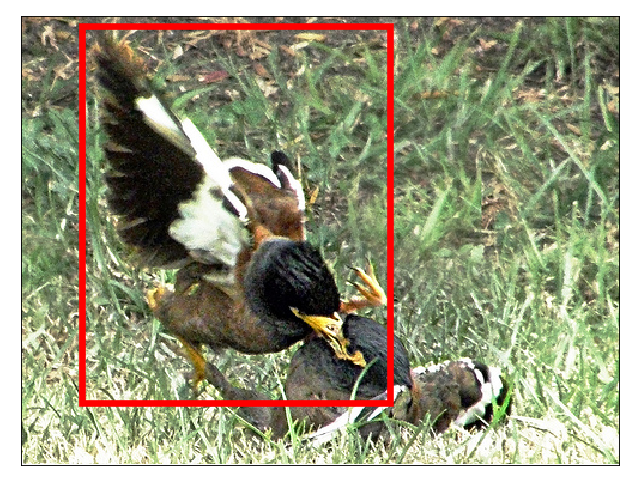
\includegraphics[scale=0.15]{images/2327551_2960743_seed_ambiguous.png} &
		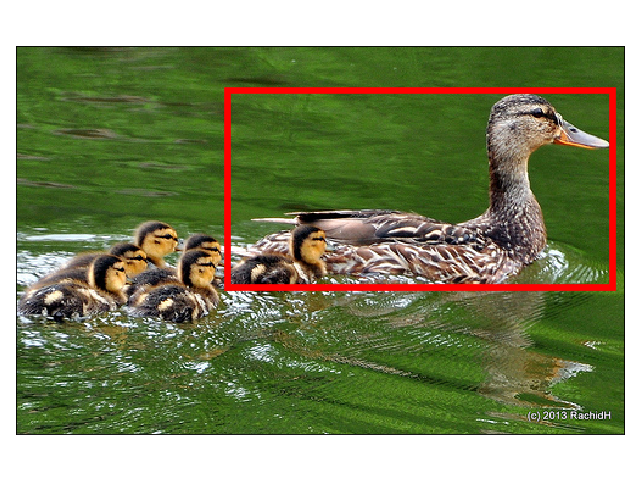
\includegraphics[scale=0.15]{images/2358126_805887_singleton_obj.png}\\
		bird\ (27),  duck\ (8) & duck (33), bird (3)\\
	\end{tabular}
	\caption{Different naming preferences for different instances of the same \category \name{duck} in \mn.\label{fig:duck}}
\end{figure}
Hence, both the single-ground-truth view of CV models and the category-level approach predominant in Psycholinguistics are insufficient for assessing the effectiveness of \lv models for human-like, entry-level object naming.
The \mn dataset was designed to help mend this gap: it consists of names entered by 36 annotators in parallel, for 25K objects in naturalistic images from \vg~\cite{krishna2016visualgenome}.
However, the name annotations of \mn have not been verified to filter out incorrect names or names for the wrong object, a problem that is in some sense the opposite of that posed by the single-ground-truth approach.

Our main contributions in this paper are (i) to run the \mn data through a rigorous annotation round to quantify both the adequacy of its names and the types of errors they contain, in order to (ii) test and compare object detection and image classification models for their ability at the task of \emph{instance-based, entry-level object naming}. More precisely, \mn enables us to define the entry-level as follows:\\
\fbox{\parbox{\columnwidth}{\textbf{Entry-level name:} the most common name given to an object instance according to \mn}}\\\\
We evaluate the effectiveness of different models on predicting these entry-level names, and our additional verification annotations enable us to understnad the kinds of mistakes each model makes (e.g.,~a `wrong' prediction may be a less preferred name as opposed to a true error).
We show that generic object classification models on their own (ResNet, Faster-RCNN and Bottom-up) already learn to provide entry-level names for objects, but also that it is possible to apply transfer learning on \mn, successfully using pre-trained features from object detection and image classification models to train entry-level naming models. 
\mw{Remark about the kinds of human errors, just as in the abstract, or some other more interesting teaser?}

%% END OF FILE %%

%Our contributions towards the task of instance-based entry-level naming in \lv and CL research are two-fold:  
%First, we provide data on object naming with real images on a large scale. 
%We take on an empirical notion of entry-level names, and define it on the instance-level, i.e., the name that humans prefer to use when calling a particular object in a real-world image.   
%We extend \mn (under submission), a dataset that provides 36 names for each of 25K objects from \vg~\cite{krishna2016visualgenome}, with information on adequacy and reference of all collected names, which affords rich analysis possibilities. 
%
%Second, we introduce the verified \mn dataset as evaluation data, and provide an extensive analysis of the ability of object detection and classification models to account for entry-level object naming in our dataset. 


\iffalse
%However, when they speak, humans in general name specific \textit{instances} of objects---actually, instances in particular situations and points of view, which may humans have prefer different names for instances of the same \category, and have them even disagree in their choice for the same instance (see also \citealt{graf2016animal}). 


%Accordingly, datasets used for object naming in Psycholinguistics use idealized drawings that correspond more to categories than to instances~\cite{+++++}.
%
%

Despite its relevance in \lv and CL, the challenge of instance-based natural naming has been overseen. 
\lv research that particularly focuses on the prediction of entry-level names is scarce, and existing work has adopted the \category-based concept of entry-level names \cite{Ordonez:2016}. 
Furthermore, existing datasets lack necessary information to make progress in \lv and CL research on this phenomenon. 
\cs{TODO@CS: EVALUATION ISSUE GOES HERE.}
\begin{itemize}
	\item resources developed in CV and \lv can be useful to study object naming. 
	\item However, they provide only one (or a few) name per object \ra no guarantee that it is the entry-level name. (We provide more, to have a robust estimate of entry-level names (as well as data on other possible names). \gbt{actually, maybe move this to the previous part? \ra differences with Psycholing, with CV resources})
	\item object naming has often been conflated with object classification in CV. \gbt{Discuss differences; mention the swan - whatever name it has in wordnet example of ordonez et al?}
	\item a big problem with this approach is that it follows a single-label evaluation. With our data, we show that often model responses are adequate even if they do not correspond to the entry-level name.
	\item we also show that object classification models ``spontaneously'' learn to provide entry-level names for objects
	\item and that it is possible to use \mn to successfully fine-tune existing object detection and classification models to predict entry-level names for objects.
\end{itemize}


This paper seeks to spur \lv and CL research on the problem of \textit{instance-based entry-level object naming}. 

Our contributions are two-fold:  
First, we provide data on object naming with real images on a large scale. 
We take on an empirical notion of entry-level names, and define it on the instance-level, i.e., the name that humans prefer to use when calling a particular object in a real-world image.   
We extend \mn (under submission), a dataset that provides 36 names for each of 25K objects from \vg~\cite{+++}, with information on adequacy and reference of all collected names, which affords rich analysis possibilities. 

\cs{I'll continue from here.}
Second, we introduce the verified \mn dataset as evaluation data that allows XXX. We provide an extensive analysis of the ability of object detection and classification models on the task of predicting the entry-level names in our dataset.


When people talk, they choose particular names for objects, such as \textit{bird} or \textit{duck} for the images in Figure~\ref{fig:duck}.
The task of \textbf{object naming} has been studied in Psycholinguistics~\cite{refs}, \gbt{Which term do you prefer, Psycholing, or CogSci? I don't care. Use same term throughout.} but has not received much attention in Computational Linguistics; we seek to remedy this situation by providing data and modeling results on this phenomenon, and in particular on \textbf{entry-level names}, defined in psycholinguistic research as the preferred name for an object~\cite{rosch1976basic,Rosch1978,jolicoeur1984pictures}: For the left object in the figure, according to our data, the entry-level name is \textit{bird}, and for the right object it is instead \textit{duck}.
%We seek to shed light into how people naturally name objects in real images, and in 


Our contributions are two-fold.
First, we provide data on object naming with real images on a large scale.
We extend \mn (under submission), a dataset that provides 36 names for each of 25K objects from \vg~\cite{+++}, with information on adequacy and reference of all collected names, which affords rich analysis possibilities. 
Our data contain object instances, corresponding more closely to the kind of visual objects that humans typically encounter, and so can potentially shed light on the instance-level factors that affect naming. 

Second, we provide an extensive analysis of the performance of object classification models on the task of predicting the entry-level names in our dataset.

As for the former, note that Psycholinguistic research on entry-level names has focused on categories, as opposed to instances:
When a subcategory is atypical, such as penguins not being very typical birds, this affects their entry-level name (it is common to call a sparrow, but not a penguin, \textit{bird}).
Accordingly, datasets used for object naming in Psycholinguistics use idealized drawings that correspond more to categories than to instances~\cite{+++++}.
However, when they speak, humans in general name specific \textit{instances} of objects ---actually, object instances in particular situations and points of view.
Our data contain object instances, corresponding more closely to the kind of visual objects that humans typically encounter, and so can potentially shed light on the instance-level factors that affect naming.
%Indeed, Psycholinguistic research has typically ignored
% The example shows two instances of the category \textsc{duck}, and when people were asked to name the highlighted object, most ($27$) people called the instance on the left \name{bird}, while \name{duck} was strongly preferred for the right instance. 
%It seems plausible that there are instance-specific factors affecting naming behavior in general.
%, and entry-level names in particular, and our data suggest that this is the case
% gbt: maybe put back a "crucially" somewhere: "Crucially, though, as we will empirically show, human object naming is \textit{instance}-dependent: It depends on the characteristics "
In particular, we validate the notion of entry-level name at the instance level:
For almost 90\% of the 25K objects analyzed, humans showed a preference for a given name (frequency of that name $>50\%$ of the valid responses).

As for the second contribution, \gbt{to be expanded; proposed structure follows; probably here only a summary and a fuller explanation later?}
% allows for an in-depth analysis of naming data as well as of naming models on the task of object naming.
\begin{itemize}
\item resources developed in CV and \lv can be useful to study object naming. 
\item However, they provide only one (or a few) name per object \ra no guarantee that it is the entry-level name. (We provide more, to have a robust estimate of entry-level names (as well as data on other possible names). \gbt{actually, maybe move this to the previous part? \ra differences with Psycholing, with CV resources})
\item object naming has often been conflated with object classification in CV. \gbt{Discuss differences; mention the swan - whatever name it has in wordnet example of ordonez et al?}
\item a big problem with this approach is that it follows a single-label evaluation. With our data, we show that often model responses are adequate even if they do not correspond to the entry-level name.
\item we also show that object classification models ``spontaneously'' learn to provide entry-level names for objects
\item and that it is possible to use \mn to successfully fine-tune existing object detection and classification models to predict entry-level names for objects.
\end{itemize}

\gbt{Below is the old text. I factored out the entry-level aspects in the previous paragraph. It should be removed from this second part.}

Objects, being members of many categories, can be called by many names (e.g.,\ a duck can be called \name{duck, bird, animal} etc.). 
In \langvis research (\lv), the choice of a particular name for an object is a ubiquitous problem---it underlies virtually all tasks that model how speakers use language to refer to objects in the world, such as image description, visual question answering, referring expression generation, etc. 
%
\lv methods are generally based on object detection or image classification models (or the visual features extracted from them) that were pre-trained towards predicting the single correct label of objects. 
The set of labels are often determined rather arbitrarily---it may contain very specific (e.g.,\ \name{goblet, gyromitra}) as well as "basic-level" labels (e.g., \name{bus}; cf.\ the label inventory of the ILSVRC challenges; \citealt{ILSVRC15}). 

This pre-training strategy has its justification in that computer vision models can learn rich, discriminative visual feature representations which capture fine-grained differences in object appearances (e.g.,\ sharp--pointed vs. slightly pointed). 
It is, however, different from predicting the natural name of an object, 
because, as has been found in numerous studies in psychology, humans have a preference towards a particular name (\textit{entry-level name}, e.g.,\ \name{duck}) when naturally calling an object  \cite{rosch1976basic,Rosch1978,jolicoeur1984pictures}. 
Entry-level names have hereby usually been considered to be an attribute of concrete \textit{concepts} (e.g.,\ penguin, duck), where the choice of a concept's entry-level name depends on factors such as its typicality with respect to its basic-level category (bird). \cs{Need to check Jolicoeur and their experiments} 
Crucially, though, as we will empirically show, human object naming is \textit{instance}-dependent---contextual visual features may humans have prefer different names for object instances of the same concrete concept, and have them even disagree in their choice for the same instance (see also \citealt{graf2016animal}). 
For example, Figure~\ref{fig:duck} shows two instances of the concept duck, and when people were asked to name the highlighted object, most ($27$) people called the instance on the left \name{bird}, while \name{duck} was strongly preferred for the right instance. 

Despite its relevance in \lv, the challenge of instance-based natural naming has been overseen, and most \lv datasets not necessarily provide enough information to make progress on the problem of modeling natural object naming (they only provide very few names). 
Research that particularly focuses on the prediction of entry-level names is scarce, and existing work has adopted the view that (i) entry-level names arise on the conceptual level, and (ii) developed specialized methods \cite{Ordonez:2016}. 
%To our knowledge, work that gives systematic insights into the ability of standard object recognition models to account for natural object naming, and in how far simple \cs{straightfoward?} re-training or transfer learning can increase this ability, is lacking. 
%

In this paper, we seek an understanding of the notion of entry-level names of instances of real-world objects in images, and to give systematic insights into the problem of retraining or fine-tuning object detection models (and features in transfer learning) such that they capture a natural vocabulary and account for linguistic preferences in naming. %, i.e.,\ the name that humans naturally prefer to call an object.  
Specifically, and in contrast to previous works, we 
(i) take on an empirical notion of entry-level names, and define it on the instance-level, i.e., the name that humans prefer to use when calling a particular object in a real-world image.   
(ii) We examine in how far standard models in computer vision, namely object detection and image classification models, do learn entry-level naming by being trained on images labeled with rather \textit{\arbitrary} (as opposed to entry-level) object names. \cs{add sth based on results - how to fine-tune or whether it's possible to fine-tune; how readily available they are to be used for transfer learning, the standard method in \lv}

We use \mn, a new dataset of real-world images, built on top of \vg, which provides an excellent resource for our study, since it was annotated with a large number\ $(36)$ of object names by means of a crowdsourcing study.

Our contributions are: 
(i) We present our extension of the \mn dataset that augments all collected object names with verification information, which allows an in-depth analysis of naming models on the task of object naming. 
(ii) Theoretical:
(a) We show that entry-level names should be derived on the instance-level as opposed to the XXX level \cs{(TO SHOW: entry-level names are different for the same "class" @Sina or @Matthijs?) (contrast to psychological studies)}
(b) We need many name annotations to derive the entry-level name (contrast to few annotations in L+V and computer vision; \cs{TO SHOW: entry-level name of an instance varies depending on the number of annotations/instance)}
(iii) Technical:
(a) Object detectors trained on "\arbitrary" natural object names do learn entry-level names to some extend (as expected: they learn the shared features leading to entry-level \cs{-- can we show that mistakes are rather class-based? i.e., tendency towards a certain name for each class?)}
(b) To predict entry-level names without annotating a huge amount of training examples, it is possible to fine-tune (iii) on \mn. We show that \cs{(say something about mistakes not made anymore). }

\fi
%%% Local Variables:
%%% mode: latex
%%% TeX-master: "acl2020_main"
%%% End:


\section{Related Work}
\label{sec:related}
%
%\paragraph{(Entry-Level) Object Naming}
%cognitive science/psychology:\\
%- levels of specificity\\
%- basic-level vs. entry-level\\ 
%- object naming studies
%
%Language + Vision:\\
%Ordonez et al., Zarriess \& Schlangen, ... \\
%- Our work: empirical notion of entry-level
%\cs{Necessary to say something about class vs. category? Otherwise I would just always use class to make things easier.}
%% SHORTENING %%Our work on natural object naming connects research in psycholinguistics, \langvis and computer vision. 
In psycholinguistics, studies of picture naming have found that humans identify objects at a preferred level of abstraction, the so-called basic-level \cite{rosch1976basic,jolicoeur1984pictures}. 
The typicality of the object with respect to this basic-level is important for determining the preferred name, i.e.\ the entry-level name: typical objects (e.g.,\ a robin) are simply named by their basic-level \category (\name{bird}), while atypical objects (e.g.,\ \name{penguin}) are preferably named by the more specific \category.
%% This strictly taxonomic view suggests that entry-level names generally hold for all instances of a \category (e.g.,\ penguin).   \mw{Not true!!}
\newcite{Ordonez:2016} adopt this and train a model to map an object's \category detected by an object recognition system to its natural name, guided by external resources like corpus statistics.
By contrast, we use \mn (details below) to directly test and fine-tune object recognition (and image classification) systems, without presupposing a taxonomical relationship between the possible names for an object.

Our approach is closer in this regard to \newcite{zarriess-schlangen:2017}, who train an object naming model from names produced in referring expressions to real-world objects.
However, they do not have access to name annotations from (many) different annotators, and they rely on simple evaluation measures (like accuracy) whereas the additional annotations we collect enable more fine-grained evaluation.
The \mn dataset on which we rely is akin in spirit to older picture naming datasets (e.g.,~\newcite{rossion2004revisiting}) but focuses on naturalistic images of real-world objects instead of prototypical line drawings.

 %\sz{maybe we should not mention the Graf paper here ... we do not look at objects in context}
 
%members of different \textit{basic-level} categories (e.g., a duck, a robin, a penguin, etc. are all members of \cat{birds}) 
% \newcite{rohde2012communicating} and \newcite{graf2016animal} investigate naming in context and find that the specificity of a name is dependent on the taxonomic relatedness of other objects in context.

%% SHORTENING %% \cs{Need to check Jolicoeur and their experiments; say sth about shared visual features}
% prototypical visual features common to all its instances (e.g.,\ apples are round, pears are ... (CHECK)). 

In Computer Vision a major focus is visual object recognition, with object classification being a core task. 
Neural image classification systems are trained to label the most salient object in an image and often use the ImageNet \cite{imagenet_cvpr09} benchmark that labels images/objects with 1,000 fine-grained classes \cite{googlenet,he2016deep}. 
These neural classifiers have proven extremely useful %% SHORTENING %%in a large range of transfer learning scenarios. They are commonly used 
as pre-trained feature extractors in object detection systems that localize objects and predict their labels \cite{fasterrcnn2015}.
For instance, a commonly used object detector in \lv is \citep{anderson2018updown}'s so-called bottom-up model, which is based on a pre-trained ResNet classifier and fine-tuned Faster-RCNN \cite{fasterrcnn2015} for object detection and classification on \vg. 
We will use pre-trained ResNet, Faster-RCNN and Bottom-up as models in this paper, extending and testing them for entry-level object naming. 

\paragraph{The ManyNames Dataset}
The \mn dataset (MN, Anonymous, under review) which builds upon object annotations in VisualGenome (VG), provides up to 36 name annotations for 25K objects in images, see e.g.\ Figure \ref{fig:duck}.
The large number of name annotations per object in \mn gives us a way to reliably derive entry-level names, defined as the most frequent name for an object instance.
Its vocabulary of all names has 7,970 types; restricted to entry-level names it has 442 types (still covering over 50\% of the objects in \vg).
	%% SHORTENING %%The vocabulary of all entry-level names in \mn contains 442 types (the vocabulary of all names is 7970), covering more than 50\% of the objects in \vg, i.e. almost 2M objects in \vg are mentioned in region descriptions with one of these 442 entry-level names.
That these objects are diverse and visually situated in real-world scenes aligns with our view that entry-level names should be characterized at an instance-level, not at the class-level.
However, our manual inspection of the \mn data revealed a range of annotation problems, e.g., annotators occasionally named an object different from the one highlighted by the bounding box, or the right object but with an incorrect name.
Although these errors are interesting human data, many of them would not occur in actual language use but are artifacts of the crowdsourcing methodology that uses simple graphical boxes to point workers to the annotation target.
%used for \mn, where there is a financial incentive to complete the task as quickly as possible.
As such they pose challenges for our research goal, which is to see whether the object-naming ability of computational models resembles that of actual language users.
To overcome these we collected a new layer of verification annotations on top of \mn, as follows.

%Current recognition benchmarks use labels (and images) from the ImageNet \cite{imagenet_cvpr09} taxonomy, but typically implement a single ground-truth label approach.
%- Object detection, using pre-trained feature representations (see next point) (localize object and predict its \textit{label}; trained with, e.g.\ more coarse-grained ImageNet labels or VG names)\\
%- Pre-trained feature representations, trained on image classification with 1000 ImageNet fine-grained labels (predict \textit{label} for most salient object in image). It predicts the class of the most salient object in an image. \\
%- Our work: can object detectors account for natural human object naming with respect to predicting the entry-level name? 

\section{Adequacy and Errors in ManyNames}
\label{sec:manynames}
%\cs{to add: footnote saying that the \mn data will be published upon acceptance of the paper.}
\begin{itemize}
\item brief intro to manynames and the verification procedure 
\item limit the analysis to aspects that are clearly and strictly related to the goals of the paper: 1)~quality of the verification data itself (inter-annotator agreement), 2)~show that most objects do in fact have a ``natural name'' (such that it makes sense to do single-label classification with those), 3)~show that we need for many annotations to establish ``natural name''. TBD: also show the distribution of human errors in the original ManyNames v.1 data?
\end{itemize}


% \begin{figure}[t]
% 	\centering
% 	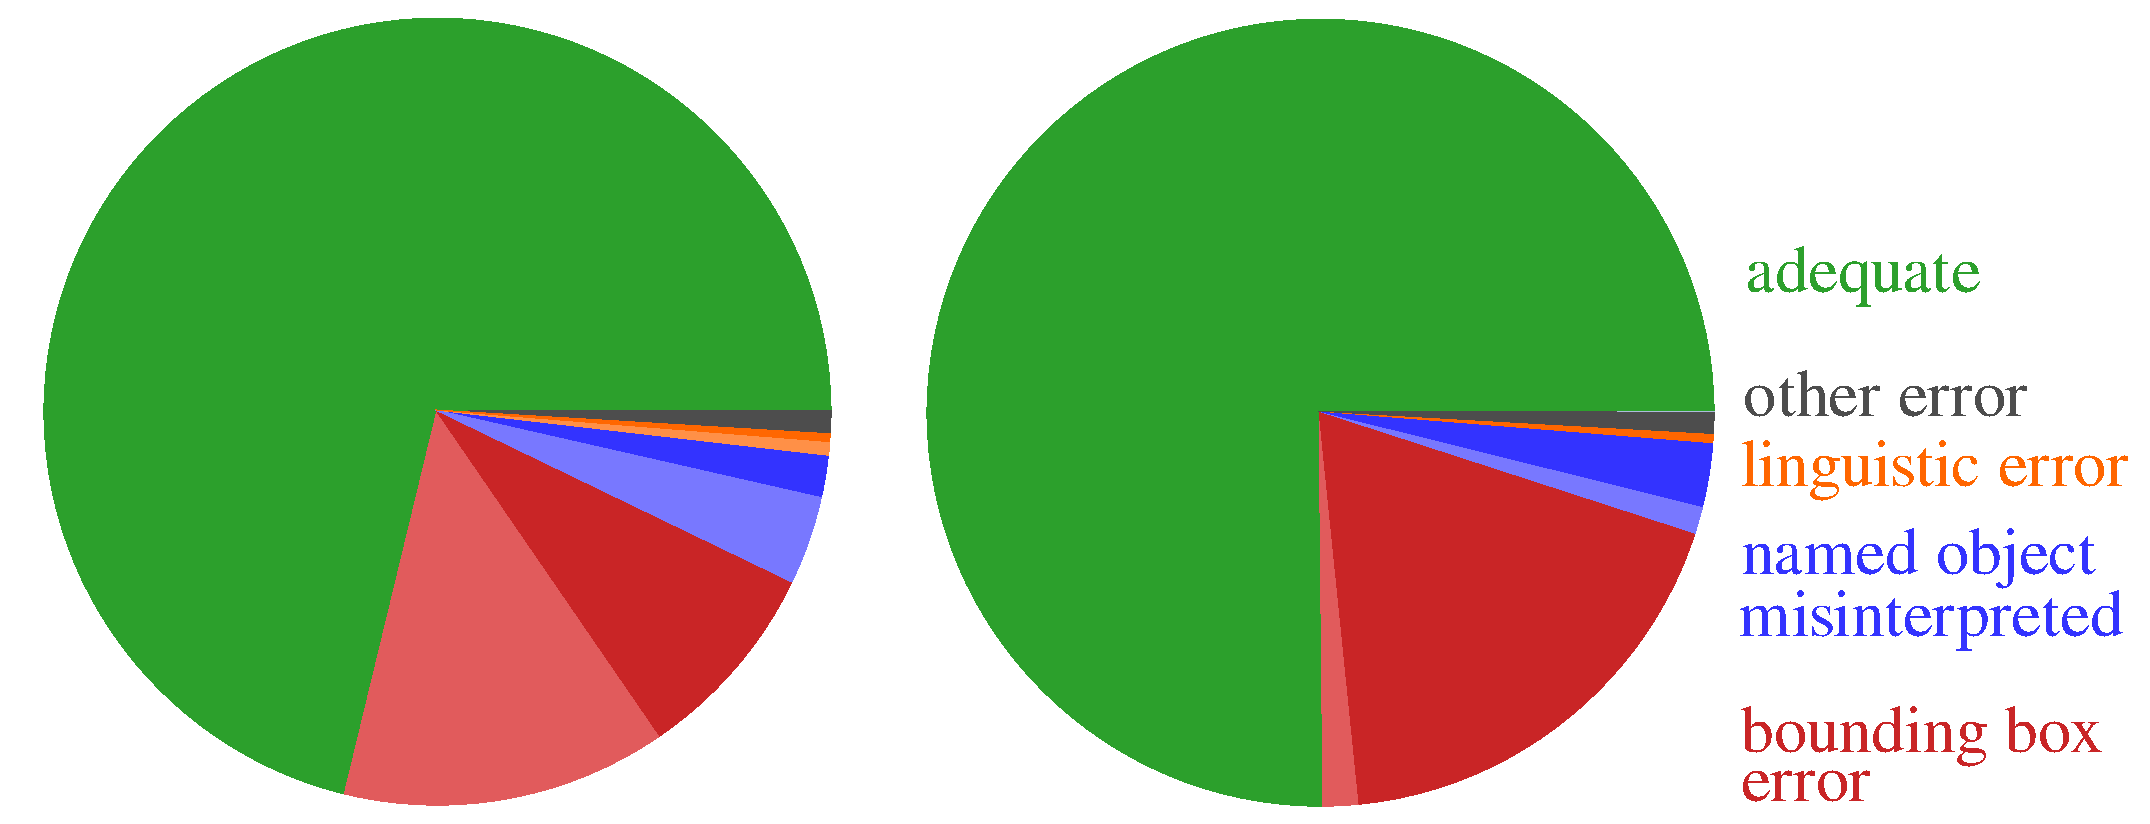
\includegraphics[width=\columnwidth]{images/verification_piechart_double.pdf}\\
% 	\hspace*{\fill}a.\hspace*{\fill}\hspace*{\fill}b.\hspace*{\fill}\hspace*{\fill}
% 	\caption{Verification results: a. counting individual annotations; b. counting image-name pairs with their aggregated scores. Lighter shade within a hue indicates slight/possible error of that type; darker shade severe error.}
% 	\label{fig:verification-piechart}
% \end{figure}


%%% Local Variables:
%%% mode: plain-tex
%%% TeX-master: "acl2020_main"
%%% End:


\section{Predicting Entry-Level Names}
\label{sec:experiments}
%% experiments.tex

Given the entry-level naming data from \mn, which extends the more \arbitrary naming data from VisualGenome (VG), we now have a variety of possibilities to train, re-train or fine-tune existing object detection or classification models, to capture natural naming.
Moreover, we can systematically vary the vocabulary for these models during training: a standard object naming vocabulary compiled from a frequency list as in \cite{anderson2018updown}, or a set of entry-level names as aggregated from the ManyNames data.
Our experiments will assess these various modeling decisions for the task of entry-level naming, in the current section by using accuracy as a standard evaluation metric.
Section~\ref{sec:analysis} will analyze the results with respect to the different types of errors identified by our verification data.
% found in the verification data in Section \ref{sec:verification}.
%We leave modeling experiments that take into account other possible names of objects for future work.

% Our goal is to experimentally obtain insights into the usefulness of computer vision object labeling models, that are commonly used for \lv methods, to account for natural human object naming. 
% Specifically, our research questions are
% \begin{enumerate}
% 	\item Do object detection models, despite being trained on \arbitrary  
% 	names, account for human object naming?\cs{repetitive}
% 	\item Can we apply simple transfer learning on \mn to train classifiers towards this naming task by utilizing pre-trained object detection or image classification model as feature extractors? Figure~\ref{fig:exp_confusions} \\
% 	\cs{move to models: -- can we learn entry-level names by fine-tuning object detection models on \mn?\\
% 		-- Can we directly learn entry-level names by fine-tuning image classification models on \mn, i.e.,\ the pre-trained features to initialize object detection models?}
% \end{enumerate}
% TO BE COVERED BY THE SUBSECTIONS BELOW:
% \begin{enumerate}
% 	\item Do models prefer the entry-level name of an object over an \arbitrary name? Table~\ref{tab:exp_VGvsMN}
% 	\item In cases of failure, do they predict alternative, but less preferred  names instead? Tables~\ref{tab:exp_overview_results}, \ref{tab:exp_alternatives}
% 	\item What phenomena of human behavior on the object naming task of \mn do the models mirror? That is, which model mistakes or confusions are due to the artificial setup of the task itself, and less a failure of the model? (Recall that \mn serves as a \textit{proxy} for natural human object naming, since annotators were asked to name a highlighted object in an image isolated from its situative context; Section~\ref{sec:manynames}) Table~\ref{tab:exp_details_wrong} (and \ref{tab:exp_errors_agreement},  \ref{tab:exp_alternatives})
% \item \cs{Not examined at the moment -- MRR and Jaccard may be re-added for this: Are valid name alternatives among the top-N predictions?}
%\item do we get different evaluation results when testing existing object classification models on preferred responses from name distributions, as compared to naming responses collected from 1-3 workers (e.g., VisualGenome)? 
%\end{enumerate}

\subsection{Experimental Setup}
\label{sect:exp_setup}

\paragraph{Data}
We split \mn into training ($21$K objects) and test data ($1,072$), where the test data corresponds to the overlap of \mn (MN) and the \vg (VG) test split used by  \newcite{anderson2018updown}. 
The target vocabulary of the test data is MN442: the $442$~entry-level names we derived from \mnshort. %the overlap of MN442 and VG ($355$ names). 
For transfer learning we train models on the ground truth entry-level names provided by \mnshort, and compare this to training on \vgshort labels. 

\paragraph{Models}
We test two object detection models trained on objects and names from the original \vg data, using the Faster R-CNN architecture \cite{fasterrcnn2015}, initialized with features that were pre-trained on $1$K~ImageNet classes with the ResNet-101 classification model \cite{he2016deep}.
We use and retrain these two models with different target vocabularies:

\begin{itemize}
\item FRCNN$_{\text{VG1600}}$: We use \citeauthor{anderson2018updown}'s  \shortcite{anderson2018updown} model\footnote{We used the code and model available at  \url{github.com/peteanderson80/bottom-up-attention}. The model is trained with an additional output over attributes, but we only use the object class prediction layer.} that is optimized for a set of $1600$~object names in \vgshort. This set was obtained by first taking the $2500$~most frequent names in \vgshort and then (manually) filtering certain names.
 \item  FRCNN$_{\text{MN442}}$: We pre-process the \vgshort data as in \citeauthor{anderson2018updown}, but restrict the object classes to the $442$~entry-level names found in \mn (Section~\ref{sect:mn_analysis}). 
For training, we use a PyTorch reimplementation of Faster R-CNN\footnote{\url{github.com/jwyang/faster-rcnn.pytorch}}
\end{itemize}

The two former models are trained on \vg, which has almost $4$~million labeled objects.
\mn is too small to train object detection models on it from scratch, which requires learning millions of parameters.
On the other hand, obtaining enough naming data to be able to estimate entry-level names for larger datasets is very costly and probably unrealistic.
Therefore, we investigate the possibility of obtaining effective entry-level naming models via transfer learning, fine-tuning existing models with \mn data.
We do so with the standard methodology of taking the last hidden layer of existing Computer Vision models as input, and train object classification models to predict entry-level names (MN442).

We experiment with two kinds of (transferred) input features, different training vocabularies (similar to the detection models above), as well as ground-truth names with which the  instances are annotated (provided by either \mnshort or \vgshort).
This yields the following $5$~transfer-learning-based naming models:
\begin{itemize}
\item FRCNN$_{\text{VG1600--VGMN}}$:
	This model extracts features from the object detection model FRCNN$_{\text{VG1600}}$\footnote{
	As experimental results will show, FRCNN$_{\text{VG1600}}$ is more effective than FRCNN$_{\text{MN442}}$, so we only use the former.
}. We expect these to be very good features for our task, as they have been obtained with the same task (object classification) and dataset (\vg).  For each object (i.e.,~bounding box) in \mn, we extract its activation features from FRCNN's last hidden layer before the output layer. The model uses the VGMN vocabulary (overlap of the full ManyNames vocabulary with VG).
  \item ResNet$_{\text{VGMN}}$: 
For comparison, we consider a much less informed input, namely the features from the ResNet-101 image classification model, that was used to initialize the FRCNN models above, and pretrained on ImageNet \cite{imagenet_cvpr09}. 
Results should of course be worse, and our aim is to assess the feasibility of using such generic object representations to obtain entry-level names. ResNet$_{\text{VGMN}}$ uses the VGMN vocabulary. It is optimized on VG or MN ground truth names respectively.
 \item  ResNet$_{\text{MN442}}$:
 A variant of ResNet$_{\text{VGMN}}$, that is trained with a vocabulary of $442$~entry-level names. It is optimized on VG or MN ground truth names respectively.
\end{itemize}
Note that these five models are optimized on the $21$K~objects in \mn. 
To predict the entry-level name of a target object~$o$, the classifier, a multi-layer neural network, is fed the object's features, and applies softmax activation to the output layer that corresponds to the target vocabulary. 

%\iffalse
%\begin{table}[t]
%	\centering
%	\small
%	\begin{tabular}{@{~}l@{~}|@{~}c@{~}|cc|cc@{~}}
%		\toprule
%		&  & \multicolumn{2}{c}{All} 
%		& \multicolumn{2}{c}{VG$\neq$MN}\\
%		&  & \multicolumn{2}{c}{($1072$)} 
%		& \multicolumn{2}{c}{($223$)}\\	
%		Model$_{\text{Vocab}}$ 
%		&  GTtrain &  VG & MN 
%		&  VG & MN \\ 
%		\midrule
%		FRCNN$_{\text{MN442}}$ & VG &  65.4 &      71.2 &   20.0 &      48.4  \\
%		FRCNN$_{\text{VG1600}}$ & VG &    67.3 &      74.5 &    19.1 &      52.9  \\
%		\midrule \midrule
%		\multicolumn{6}{c}{Classifiers: Transfer learning on MN}\\
%		Features$_{\text{Vocab}}$ &   \\
%		\midrule 
%		FRCNN$_{\text{VG1600}}$$_{\text{-VGMN}}$ & MN &    70.8 &      80.6 &    13.8 &      60.4  \\ 
%		\midrule
%		ResNet$_{\text{VGMN}}$ & MN  & 60.9 &  68.6 &  13.8 & 50.2  \\
%		
%		ResNet$_{\text{MN442}}$ & MN &            61.7 &              69.6 &                        13.8 &              50.7 \\
%		ResNet$_{\text{VGMN}}$  &   VG &  62.4 &              62.9 &              28.4 &              31.1  \\
%		%ResNet$_{\text{VGMN}}$\_4ep  &   VG &  62.4 &              62.9 &              28.4 &              31.1  \\
%		%ResNet101$_{\text{VGMN}}$\_8ep & VG &            63.9 &              62.6 &          34.2 &              28.0 \\
%		ResNet$_{\text{MN442}}$ & VG  &            63.7 &              63.7 &                  30.7 &              31.1  \\
%		\bottomrule
%	\end{tabular}
%	\caption{Model accuracy (in \%) on the \mn test objects. Vocab denotes the dataset used to induce the target vocabulary for training (the numbers give the size of the vocabulary). GTtrain gives the dataset that provides the ground truth labels during training, and VG and MN for testing \label{tab:exp_VGvsMN}.}
%\end{table}
%\fi
%\paragraph{Measures}


\subsection{Results}
\label{sect:exp_results}

Table \ref{tab:exp_VGvsMN} shows the accuracy of the models on the \mn test data\footnote{ResNet$_{\text{VGMN}}$ with MN is comparable to its couterpart.}. 
We compare model effectiveness on predicting the entry-level name (column MN) against predicting the VG name. 
%We therefore consider an object's VG name less likely to represent the entry-level name than its MN name. 

% and furthermore report results on the test instances where the two names differ (block VG$\neq$MN). 
%Note that the VG names were derived on the basis of a few annotations per object only, and, as shown in Section~\ref{sect:mn_analysis}, even ``just'' $10$ or $20$ names sufficiently likely yield an entry-level name for only $68\%$ or $78\%$ instances, respectively.  
%We therefore consider an object's VG name less likely to represent the entry-level name than its MN name. 
% \gbt{add motivation for the latter, and make sure we address this when we discuss results; else, remove.}. 
%\cs{Left as items for the sake of a better overview for now}

\begin{table}[t]
	\centering
	\small
	\begin{tabular}{@{~}l@{~}|@{~}c@{~}|cc@{~}}
		\toprule
		&  & \multicolumn{2}{c}{GTtest} \\
		Model$_{\text{Vocab}}$ &  GTtrain &  VG & MN  \\ 
		\midrule
		FRCNN$_{\text{MN442}}$ & VG &  65.4 &      71.2   \\
		FRCNN$_{\text{VG1600}}$ & VG &    67.3 &      \textbf{74.5} \\
		\midrule \midrule
		\multicolumn{4}{c}{Classifiers: Transfer learning on MN}\\
		Features$_{\text{Vocab}}$ &   \\
		\midrule 
		FRCNN$_{\text{VG1600}}$$_{\text{-VGMN}}$ & MN &    \textbf{70.8} &      \textbf{80.6}  \\ 
		\midrule
		%ResNet$_{\text{VGMN}}$ & MN  & 60.9 &  68.6   \\
		
		ResNet$_{\text{MN442}}$ & MN &            61.7 &              69.6  \\
		ResNet$_{\text{VGMN}}$  &   VG &  62.4 &              62.9  \\
		%ResNet$_{\text{VGMN}}$\_4ep  &   VG &  62.4 &              62.9 &              28.4 &              31.1  \\
		%ResNet101$_{\text{VGMN}}$\_8ep & VG &            63.9 &              62.6 &          34.2 &              28.0 \\
		ResNet$_{\text{MN442}}$ & VG  &            63.7 &              63.7   \\
		\bottomrule
	\end{tabular}
	\caption{Model accuracy (in \%) on the \mn test objects. Vocab denotes the dataset used to induce the target vocabulary for training (the numbers are vocabulary size). GTtrain gives the dataset providing the ground truth labels for training, and GTtest for testing \label{tab:exp_VGvsMN}.}
	\vspace{0ex}
\end{table}

A pervasive trend is that all models perform better 
at predicting the entry-level name (MN) than the VG name (VG), regardless of which vocabulary (Vocab) and which ground-truth (GTtrain) they were trained on.  
Note that the VG names were derived on the basis of a few annotations per object only, and, as shown in Section~\ref{sect:mn_analysis}, is not enough to robustly estimate entry-level names. 
%, even ``just'' $10$ or $20$ names sufficiently likely yield an entry-level name for only $68\%$ or $78\%$ instances, respectively. 
%The results therefore indicate that, even when not trained to do so (FRCNN$_{\text{VG1600}}$), models tend to predict entry-level names.
The results therefore indicate that the even the FRCNN detection models do learn entry-level naming, despite not trained being to do so, with an accuracy of up to~$74.5$\%.

 The overall best model is FRCNN$_\text{VG1600}$$_\text{-VGMN}$ (the Vanilla classifier with FRCNN$_\text{VG1600}$ features, trained on  \mn). 
 Transfer-learning on entry-level names also helps in the original task of predicting VG names---FRCNN$_\text{VG1600}$$_\text{-VGMN}$ also improves in the VG evaluation ($70.8\%$~accuracy, vs.~$67.3\%$).
 % [CS] we need to do stat. significance tests
 %
As expected, the classifiers using ResNet features are the least effective, but considering that they were trained on a fraction of FRCNN's training size using a simple Vanilla classifier, in contrast to a fully-fledged CNN architecture of the FRCNN object detectors, the drop in effectiveness on entry-level naming (column MN, GTtrain MN) is decently low. 
%This confirms what we observed on the FRCNN results. 
%
In sum, we find that models learn entry-level naming when being trained on \arbitrary naming data, obtaining better results on entry-level prediction than VG name prediction for the same instances, and that they benefit from being trained on entry-levels using transfer learning. Comparing the target vocabulary, MN442 and VG1600/VGMN, we see that the restriction on a smaller, but empirically derived vocabulary of entry-level names only, is not beneficial, with all MN442 models being worse or comparable to VGMN/VG100.

\subsection{Discussion}
\label{sect:exp_discussion}

%To date, little research has been done on how to finetune and calibrate the \textit{vocabulary} of object detection and classification models from Computer Vision, for purposes of \lv.
As Section~\ref{sec:manynames} showed, object naming is a linguistically complex phenomenon which exhibits a fair amount of agreement and also variation and potential errors. 
Hence, it is striking that even models that are trained on (a lot of) \arbitrary names capture entry-level naming to a good extent.
However, our results also suggest that current \textit{evaluation} methods might not be very reliable when applied on \arbitrary names, probably punishing models for `errors' that actually constitute plausible alternatives.
The next section elaborates on this and proposes a fairer assessment of naming quality.


%\iffalse
%\cs{under construction}
%\begin{itemize}
%	\item Object detection models in CV have different goal than L+V object recognition models (see related work--former is on labels, latter on predicting natural language). 
%	However, the former, pre-trained towards labels, are the backbone / used as feature extractors for the latter.
%	\item ... 
%	\item As we explained, there is a high variation of object names, and objects may be named by multiple alternative names (\cs{vocab size MN vs. vocab size VG for same object set}). 
%	Yet, humans usually have a clearly preferred name for individual object instances (and the set of those is relatively small)--humans agree on a particular name for an instance (entry-level name).
%	\item Hence, to model human object naming, datasets with many/dozens of annotations for the same instance are required. 
%	\item We argue that such datasets are more reliable in that they provide empirically derived preferred names (entry-level names), and richer--the provide valid name alternatives. 
%	\item But since their elicitation is expensive and time-consuming, it is not realistic to create training datasets of dozens of object names for pre-training features with CV models, which need a huge amount of training data. 
%\end{itemize}
%\fi

%\iffalse
%We propose to use datasets of object names for evaluating models on the task of object naming (depending on results: also valuable for comparing object detection/image classification models).
%Specifically, we analyse object detection [and classification] models on the task of human object naming, using the \mn dataset as test data:\\
%Can object detection models, trained on arbitrary names, account for human object naming?
%\begin{itemize}
%	\item Do they predict the entry-level name?
%	\item Are valid name alternatives among the top-N predictions?
%x	\item Do models make similar mistakes as humans when being faced with the task of naming highlighted objects in images [i.e.,\ the artificial setup of object naming for data annotation]?\\
%	-- naming an alternative object (maybe more salient)\\
%	-- predicting a semantically related name
%	%do we get different evaluation results when testing existing object classification models on preferred responses from name distributions, as compared to naming responses collected from 1-3 workers (e.g., VisualGenome)? 
%	\item Can we use \mn as fine-tuning dataset? (Here: only Vanilla model)\\
%	-- can we learn entry-level names by fine-tuning object detection models on \mn?\\
%	-- Can we directly learn entry-level names by fine-tuning image classification models on \mn, i.e.,\ the pre-trained features to initialize object detection models?
%\end{itemize}
%\fi

%\iffalse
%OLD TABLE WITH MORE MEASURES
%
%\begin{table*}[t]
%	\centering
%	\small
%	\begin{tabular}{l|c|r@{~}r@{~}r@{~}r@{~}r@{~}r@{~}r|@{~}r@{~}r@{~}r@{~}r@{~}r@{~}r@{~}r@{~}}
%		\toprule
%		&   & \multicolumn{6}{c}{All Test Images ($\#$)} 
%		& \multicolumn{6}{c}{VG$\neq$MN Images ($\#$)}\\	
%		Model$_{\text{Vocab}}$	 
%		&  GTtrain &  =VG & =MN & $\in$MN  & KL & J & MRR & AvgMRR 
%		&  =VG & =MN & $\in$MN  & KL & J & MRR & AvgMRR\\ 
%		\midrule
%		FRCNN--MN442 & VG &            65.4 &              71.2 &                85.6 &         1.0 &             69.8 &          0.8 &             0.7 &            20.0 &              48.4 &                78.7 &         1.4 &             60.4 &          0.7 &             0.5 \\
%		FRCNN--VG2500 & VG \\
%		FRCNN$_{\text{VG1600}}$ & VG &            67.3 &              74.5 &                89.2 &         0.6 &             74.3 &          0.8 &             0.7 &            19.1 &              52.9 &                86.2 &         0.8 &             69.4 &          0.7 &             0.6 \\
%		\midrule \midrule
%		& \multicolumn{12}{c}{Classifiers: Fine-tuning pre-trained image features on \mn}\\
%		Features$_{\text{Vocab}}$ & GTtrain  \\
%		\midrule 
%		FRCNN$_{\text{VG1600}}$$_{\text{VGMN}}$ & MN &            70.8 &              80.6 &                90.1 &         4.7 &             62.0 &          0.8 &             0.6 &            13.8 &              60.4 &                85.8 &         4.6 &             47.3 &          0.7 &             0.5 \\ 
%		FRCNN$_{\text{VG1600}}$--MN442 &  MN \\
%		\midrule
%		ResNet101$_{\text{VGMN}}$ & MN  &            60.9 &              68.6 &                77.9 &         4.9 &             56.4 &          0.8 &             0.6 &            13.8 &              50.2 &                73.3 &         4.7 &             42.9 &          0.6 &             0.4 \\
%		
%		ResNet101--MN442 & MN &            61.7 &              69.6 &                78.9 &         4.9 &             57.4 &          0.8 &             0.6 &            13.8 &              50.7 &                73.8 &         4.6 &             45.1 &          0.6 &             0.5 \\
%		ResNet101$_{\text{VGMN}}$\_4ep  &   VG &  62.4 &              62.9 &                75.0 &         5.0 &             53.7 &          0.7 &             0.6 &            28.4 &              31.1 &                64.9 &         4.8 &             39.1 &          0.4 &             0.4 \\
%		ResNet101$_{\text{VGMN}}$\_8ep & VG &            63.9 &              62.6 &                75.6 &         5.0 &             53.9 &          0.7 &             0.6 &            34.2 &              28.0 &                66.2 &         4.9 &             39.7 &          0.4 &             0.4 \\
%		ResNet101--MN442 & VG  &            63.7 &              63.7 &                76.6 &         5.0 &             55.4 &          0.7 &             0.6 &            30.7 &              31.1 &                67.1 &         4.8 &             41.0 &          0.4 &             0.4 \\
%		\bottomrule
%	\end{tabular}
%	\caption{Target vocabulary in test data: MN442. Vocab denotes the dataset from which the target vocabulary for training was induced (the numbers give the size of the vocabulary). GTtrain denotes the dataset from which the ground truth labels are obtained during \textit{training}. MRR is mean reciprocal rank; J is Jaccard score. Note that we considered all name responses in MN, including those with $\text{count}(name)<2$\label{tab:entrylevels}. }
%\end{table*}
%
%
%\begin{table*}[t]
%	\centering
%	\small
%	\begin{tabular}{l@{~}|rrrr}
%		\toprule
%		... \\
%		\midrule
%		Domain	 & ... \\ 
%		\midrule
%		All           \\
%		home           \\
%		food           \\
%		buildings      \\
%		vehicles       \\
%		animals\_plants \\
%		clothing       \\
%		people         \\
%		\bottomrule
%	\end{tabular}
%	\caption{RESULTS FOR SELECTED MODELS \label{tab:domains_bestmodel}}
%\end{table*}
%
%% \subsection{[TBC] Generalization Ability: OpenImages}
%% \label{sect:exp_openimages}
%% Question: Can models trained towards \mn generalize to other, related datasets? Here: OpenImages. \cs{[Increase coverage with zero-shot learning?]}\
%
%% Models compared: FRCNN$_{\text{VG1600}}$ vs. FRCNN$_{\text{MN442}}$ vs. ResNet101--XX (best Vanilla).
%\fi


%%% Local Variables:
%%% mode: latex
%%% TeX-master: "acl2020_main"
%%% End:
Largely same content, clarified. With one exception: I'd introduce two evaluation setups: 1) single label, 2) one that counts all valid names as correct. 

\section{Analysis of Model Naming Behavior}
\label{sec:analysis}
%%\gbt{Points to discuss in the paper, as discussed with Carina May 16:}
%
%\begin{itemize}
%\item Super high variance in the agreement. Higher agreement for instances, lower for classes. Suggests systematicities at the instance level that do not depend on the class. Hypothesis, supported by qualitative analysis (Figure 3): relevance of visual perceptual factors. E.g.: saliency, background/foreground (desk-keyboard; bridge-train); ``angle'' from which the object is shown (see girl-t-shirt example); \dots In addition, we also find aspects discussed by Psycholing, but at the level of the instance: Typicality (see truck-bus example, bridge-dock, bench-seat). 
%\item Forget about WordNet.
%\item Implications for lang\&vision: 1) synset classification won't do (if the goal is to predict/label an object); 2) name classification won't do either; 3) ``mistakes'' done by models are also done by humans -- role of referential uncertainty.
%\end{itemize}


In this section, we investigate to what extent names annotated in VisualGenome and elicited in ManyNames can be considered canonical, i.e. to what extent speakers agree in their naming choices.
Whereas traditional picture naming studies typically use a prototypical image per category (see Figure~\ref{fig:picture_naming}) and, hence, are mostly interested in the agreement on concept or category-level, we carry out an analysis on two different levels: First, we will look at instances and see to what extent names overlap for the same object. 
Second, we will use the existing annotation of names in VisualGenome to analyze agreement on the level of classes.
\begin{figure}[t]
	\centering
	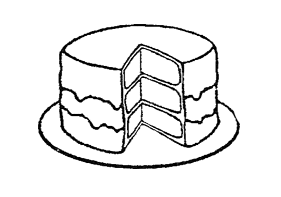
\includegraphics[scale=.5]{figures/snodgrass_vanderwart_cake_042.png}
	\caption{Example of a picture of \textsl{cake} used in traditional picture naming studies (REF to Vanderwart \& Snodgrass) \label{fig:picture_naming}}
\end{figure}

\subsection{Names, instances, classes}

First of all, to see whether objects in ManyNames bear a canonical name, we simply count how many different names (i.e.\ types) are given to instances, and to all instances that have the same synset annotated in VisualGenome. 
As the data is collected via crowdsourcing and a certain amount of noise is to be expected, we apply different frequency thresholds on the response sets for instances and synsets.
Figure \ref{fig:ntypes} shows the cumulative histograms for type counts, obtained with different thresholds (from 1 to 6).
Without any frequency thresholding, the proportion of instances and classes that have a single name annotated is small, i.e.\ below 10\% in both cases. When raising the threshold up to a minimum of 4 occurences in the response set  for instances (meaning more than 10\% of the 36 annotations), the proportion of objects that really only have a single name annotated is considerably higher, but still below 50\%.
Thus, as expected in a free annotation scenario, the MN data contains a certain number of low-frequency responses.
The fact that even after applying a relatively strict frequency filter most objects have more than one name annotated indicates that there is a non-negligible  level of variation when different speakers name the same object.

The amount of variation increases substantially when looking at the number of names we find for different synsets in Visual Genome, as is indicated by the histogram for type counts of synsets in Figure \ref{fig:ntypes}.
Here, we observe that the rise of the curve is much less steep than for instances and, generally, there are many synsets with more than 10 or even 20 different name types, even after applying the frequency threshols.

\begin{figure*}
\begin{minipage}[b]{0.4\linewidth}
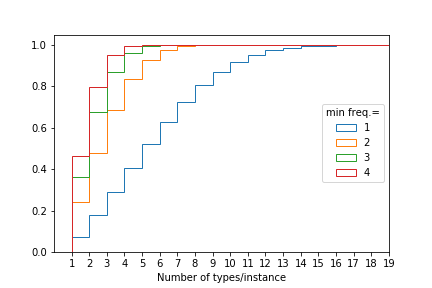
\includegraphics[scale=.4]{Figures/types_instances.png}
\end{minipage}
\begin{minipage}[b]{0.6\linewidth}
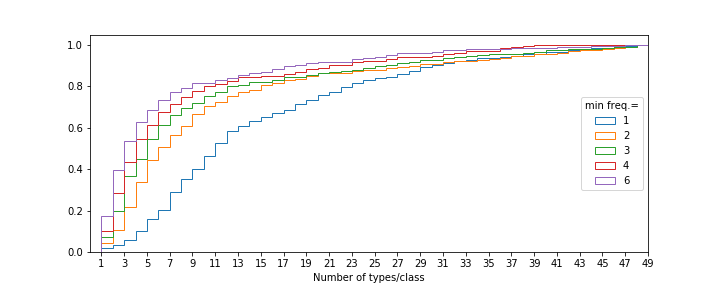
\includegraphics[scale=.4]{Figures/types_classes.png}
\end{minipage}
 \caption{\label{fig:ntypes} Cumulative histograms for number of types found for instances and classes, based on different frequency tresholds (applied on the level of instances and classes respectively)}
\end{figure*}


\subsection{Agreement}

We compute the following agreement measures:

\begin{itemize}
\item \textbf{\% top}: the average relative frequency of the most frequent response (shown in percent)
\item \textbf{$H$}: the $H$ agreement measure used previously in the psycholinguistic literature
\cs{How is this defined?}
\begin{equation}
H = \sum_{i=1}^k p_i\ log_2(1/p_i)
\end{equation}

\item \textbf{N}: the average number of types in the response set of ManyNames
%\item \textbf{N$_{>1}$}: the average number of types, excluding types that have been annotated only once
\cs{alternatively we could show a plot going from 1 to, let's say, $>10$}
\item \textbf{top=VG}: the proportion of items where the top response in ManyNames corresponds to the VisualGenome name
\item \textbf{\% VG}: the average relative frequency of the VisualGenome name in the response set

\end{itemize}

For measuring \textbf{instance-level agreement}, we consider all names annotated for an object as a response set and then average over these response sets. Furthermore, we compute \textbf{class-level agreement} by merging the response sets for all objects that have the same synset (given for the original VisualGenome name) and compute the measures over these aggregated response sets.
\gbt{@Sina, what are the synsets that you got here? Are they collection nodes, or the synset of the VG name as annotated in VG?}


Table \ref{tab:agree} shows the analysis of the instance-level and category-level agreement.
On the instance-level, our annotators achieve a fair amount of overlap in their object naming choices. 
Thus, for roughly 70\% of our objects (\textbf{std=?}), the most frequent response in ManyNames corresponds to the original VisualGenome name and, similarly, the average frequency of the top response is also 70\%. 
%Generally, this seems to suggest that indeed many objects in our data set have a canonical name. 
\sz{For NLP people, this looks like a good agreement (given that people were free to type what they wanted). For vision people who might think of it as an object labeling task, this would be pretty low/bad agreement.}
At the same time, the average number of name types per object (5.7, or 2.9 when excluding low-frequency types in each response set) suggests that there is a stable amount of naming variants that is elicited for instances. 
Furthermore, the agreement varies quite considerably among domains \cs{refer to std}:  in the animal domain, which is often discussed in the object naming literature, annotators achieve a very stable and robust agreement of over 90\% and an $H$ agreement which comes close to 0 (where 0 is perfect agreement). 
The people domain, on the other hand, is subject to much more variation and agreement is dramatically lower here, and comes close to 50\% for \% top.



%\gbt{Super-interesting results.}
Finally, the category-level agreement figures tell yet another story: when aggregating the responses for all objects with the same VisualGenome synset, we obtain on average 30 types (with $N_{>1})$, i.e. variants of the original VG class. 
Surprisingly, here, only 32.7\% of the aggregated response sets still have the VG name as the most frequent response, which means that for 70\% of the VG names, annotators in ManyNames, on average, prefer a different name.  
Likewise, the relative frequency of the top response drops considerably and $H$ increases from 1.3 for instance-level agreement to 2.4 on object-level agreement.  
%\cs{Can we say more about what's going on in the people and vehicles domain, category-level, top=VG? E.g., put corresponding examples in Tab.\ref{tab:qual}}
%

\subsection{Variation and WordNet}

Previous work on large-scale collections of labels or names of objects has (explicitly or implicitly) assumed that once naming data is canonical, linguistic alternatives of the canonical name can simply be retrieved from existing taxonomies like e.g.\ WordNet. 
%If this was indeed the case, it would be feasible (and probably even desirable) to canonicalize object names during dataset collection, without loosing too much information about linguistic variations in natural object naming scenarios (like e.g.\ referring expression generation).
Hence, in this section, we investigate to what extent the variation in object naming that we find in our MN data set (see previous Section) is covered by WordNet.
%In this section, we take a closer look at the lexical variation we observe in our data set. 
We analyze the data points where participants attributed different names to the same object and extract a set of  pairwise \textbf{naming variants}. These naming variants correspond to pairs of words that can be used interchangeably to name certain objects.
For each object, we extract the set of naming variants $s = \{ (w_{top},w_2), (w_{top},w_3), (w_{top},w_4),... \}$  where $w_{top}$ is the most frequent name annotated for the object and $w_2 ... w_n$ constitute the less frequent alternatives of $w_{top}$.  The  \textbf{type frequency} of a naming variant $(w_{top},w_x)$ corresponds to the number of objects where this variant occurs. The \textbf{token frequency} of $(w_{top},w_x)$ corresponds the count of all annotations where $w_x$ has been used instead of $w_{top}$.
In Table \ref{tab:exvariants}, we show the naming variants with the highest raw token frequency for each domain. 
The naming variants can be grouped according to their lexical relation, as follows:

\begin{itemize}
\item \textbf{synonymy}: e.g.\ aircraft vs. airplane 
\item \textbf{hyponymy}: e.g.\ man vs. person
\item \textbf{co-hyponymy}: e.g.\ swan vs. goose
\item \textbf{no relation}: e.g.\  desk vs. apple
\end{itemize}

\begin{table}
\small
\centering
\begin{tabular}{lcc}
\toprule
         relation & \% types & \% token \\
\midrule
% meronym &  0.1 &  0.2 \\
% holonym &  0.1 &  0.4 \\
 synonym &  1.1 &  1.1 \\
 hyponym &  2.2 &  3.8 \\
 co-hyponym &  3.1 &  5.9 \\
 hypernym &  10.5 &  27.7 \\
 word-not-covered &  10.6 &  2.6 \\
 rel-not-covered &  72.2 &  58.3 \\
\bottomrule
\end{tabular}
\caption{Lexical relations of naming variants in MN to annotated VG synset, averaged over synsets}
\label{tab:rel}
\end{table}


Research on object naming following the idea of entry-level categories has, essentially, exclusively looked at names that stand in a hierarchical relation (i.e.\ hyponymy/hypernymy).

We use WordNet to extract lexical relations between the naming variants in our data set.
Unfortunately, this means that we have to exclude a certain portion of the data as either (i) one of the name is not covered in WordNet, (ii) we cannot find a lexical relation between the two names (see below). Also, we had to be relatively permissive with respect to the definition of hyponymy/co-hyponymy. 
For instance, to analyze \textit{giraffe} as a hyponym of \textit{animal} we have to look at the closure of the hyponyms of \textit{animal} with a depth of 8 (in WordNet).
\sz{should we call this co-hyponymy or co-hierarchical relation?}

\sz{include Table that reports counts of the naming variants, coverage in WordNet etc.} \gbt{I think it'd be best to put the out-of-wordnet info in the Lexical relations table -- this way we have everything in one place.}

Table \ref{tab:rel} shows the distribution of lexical relations for those naming variants that we were able to analyze with WordNet.
Both in terms of their types and token frequency, the naming variants that instantiate a (loose) co-hyponymy relation are by far the most frequent.
\sz{discuss in more detail, discuss: to what extent is this an artefact of WordNet?}
This is really interesting: most research on object naming, to date, has focussed on hyponymy/hypernymy, i.e. variation that relates to hierarchical relations between object names.
Our data suggests that co-hierarchical variation is really important too.



%\subsection{Qualitative Analysis}

%\sz{put qualititative discussion here} Table \ref{tab:qual} shows examples for canonical and non-canonical VG names in our data set, where canonical means that the name was the top response in the aggregated response set in ManyNames.

%\begin{table}
%\small
%\begin{tabular}{lp{4.8cm}r}
%\toprule
%VG name &  top5 MN names &  n$_{obj}$  \\
%\midrule
%\multicolumn{3}{c}{\it Canonical VG names with max agreement in MN}\\
% giraffe &  giraffe (96.8), animal (1.2), zebra (0.4), camel (0.3), pole (0.1) &  915 \\
% zebra &  zebra (96.3), animal (1.0), giraffe (0.9), horse (0.2), microwave (0.2) &  461  \\
% cat &  cat (94.8), animal (0.9), kitten (0.8), dog (0.4), laptop (0.2) &  754\\
%\midrule
%\multicolumn{3}{c}{\it Canonical VG names with min agreement in MN}\\
% booth &  booth (19.3), table (12.3), phone booth (9.8), bench (6.7), building (4.4) &  11 \\
% cabbage &  cabbage (21.4), lettuce (17.0), hotdog (11.9), food (10.7), salad (10.4) &  9 \\
% robe &  robe (22.1), shirt (16.8), jacket (13.3), dress (5.7), clothing (3.2) &  19 \\
%  \midrule
%  \multicolumn{3}{c}{\it Non-canon. VG names with max agreement in MN}\\
% sedan &  car (88.4), wheel (3.1), vehicle (2.3), automobile (1.3), dog (0.8) &  11 \\
% pony &  horse (83.9), pony (9.1), animal (2.9), donkey (1.1), cow (1.1) &  8 \\
% necktie &  tie (81.4), necktie (10.2), shirt (4.6), ties (1.5), jacket (0.5) &  11 \\
% \midrule
%   \multicolumn{3}{c}{\it Non-canon. VG names with min agreement in MN}\\
% shelter &  umbrella (9.7), shelter (8.8), roof (8.0), tent (7.1), building (6.8) &  10 \\
% bath &  shower (13.3), elephant (9.9), birdbath (8.1), water (7.2), trough (7.2) &  10 \\
% vegetable &  food (15.7), broccoli (13.1), sandwich (10.6), salad (9.3), pizza (7.8) &  25 \\
%\bottomrule
%\end{tabular}
%\caption{Examples for VisualGenome (VG) names and their most frequent corresponding responses in ManyNames (MN; percentages shown in brackets). ``Canonical'' means that the VG name is the top name in MN, and non-canonical vice versa.}
%\label{tab:qual}
%\end{table}

\begin{figure*}
\begin{minipage}[b]{0.5\linewidth}
{\footnotesize
\setlength{\tabcolsep}{1pt}
\begin{tabular}{p{4cm}|p{4cm}|p{4cm}|p{4cm}}
%\textbf{desk} &  \raisebox{-\totalheight}{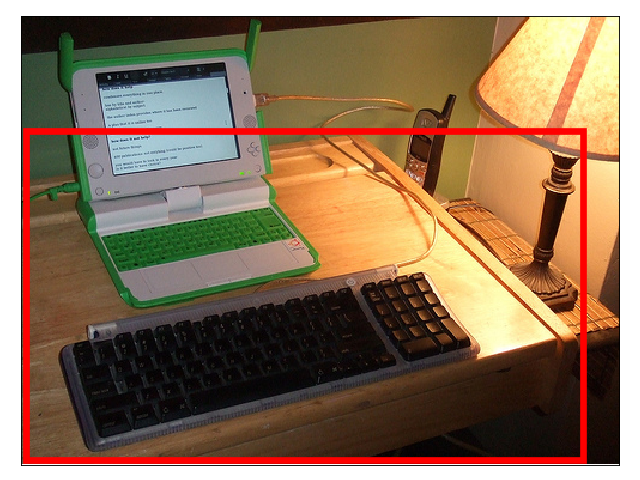
\includegraphics[width=0.9\linewidth]{figures/2320949_1048853_singleton_obj.png}} MN: keyboard  &
%\raisebox{-\totalheight}{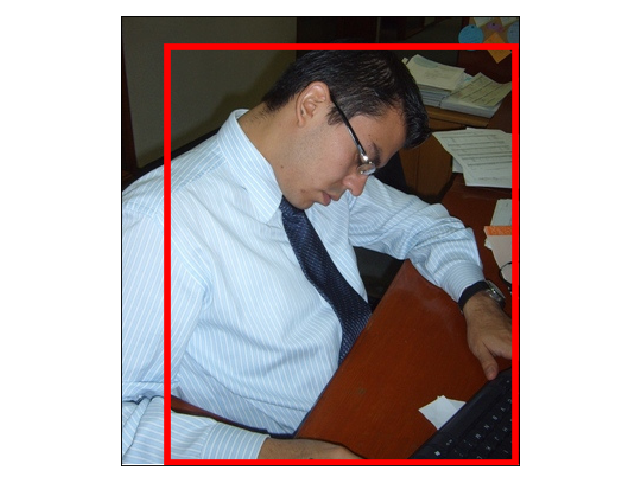
\includegraphics[width=0.9\linewidth]{figures/2343219_926143_supercat_unique.png}}  MN: desktop &
%\raisebox{-\totalheight}{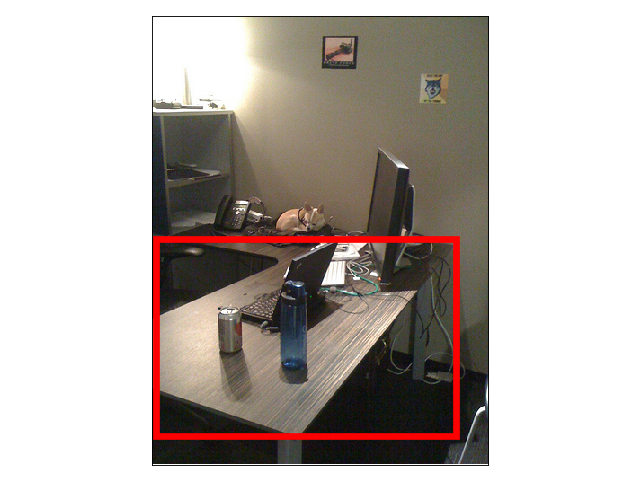
\includegraphics[width=0.9\linewidth]{figures/2354847_1742687_seed_ambiguous.png}} MN: computer \\
%\textbf{bench} &  \raisebox{-\totalheight}{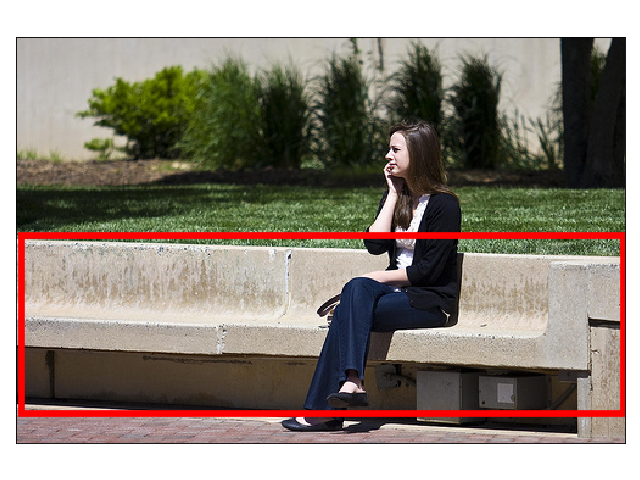
\includegraphics[width=0.9\linewidth]{figures/2350360_1042111_supercat_unique.png}} MN: table  &
%\raisebox{-\totalheight}{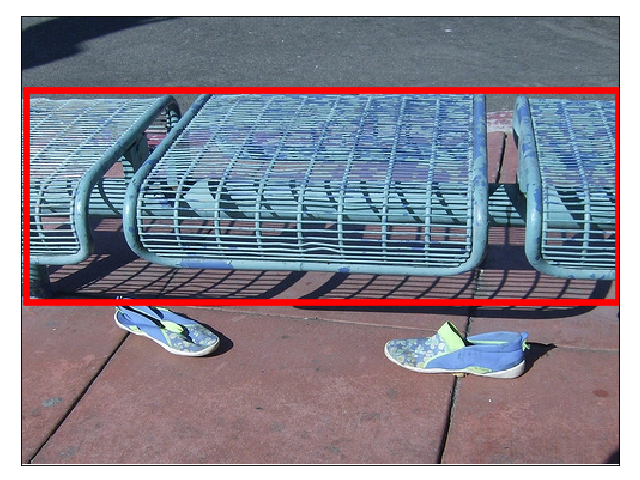
\includegraphics[width=0.9\linewidth]{figures/2389358_1261752_singleton_obj.png}}  MN: seat &
%\raisebox{-\totalheight}{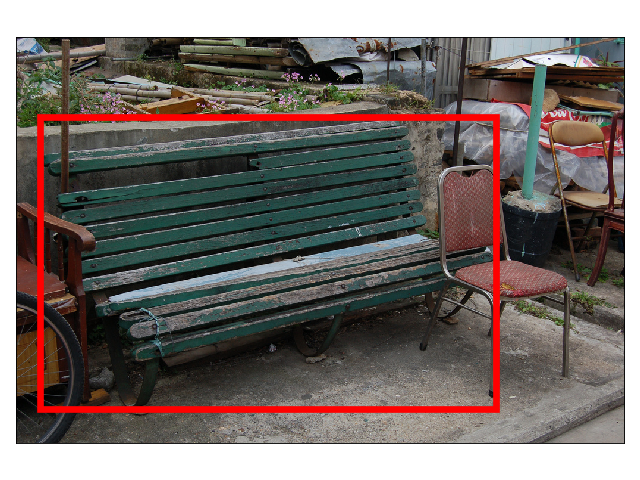
\includegraphics[width=0.9\linewidth]{figures/1593011_2063521_singleton_obj.png}} MN: wood \\
\multicolumn{4}{c}{\textbf{VG: sandwich}}\\
 \raisebox{-\totalheight}{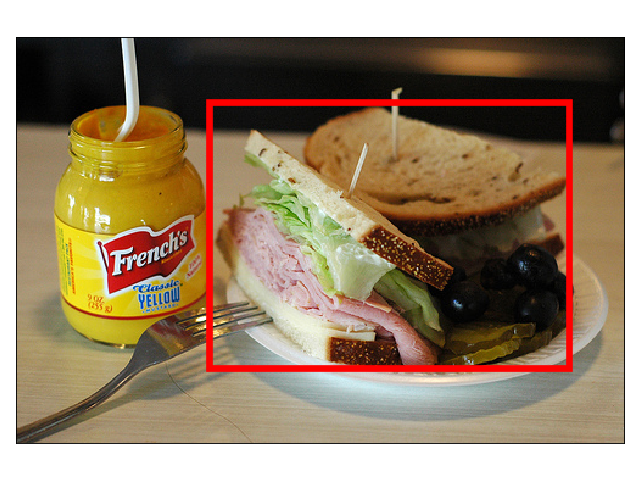
\includegraphics[width=0.9\linewidth]{figures/2339876_3928476_supercat_unique.png}} sandwich (34) &
\raisebox{-\totalheight}{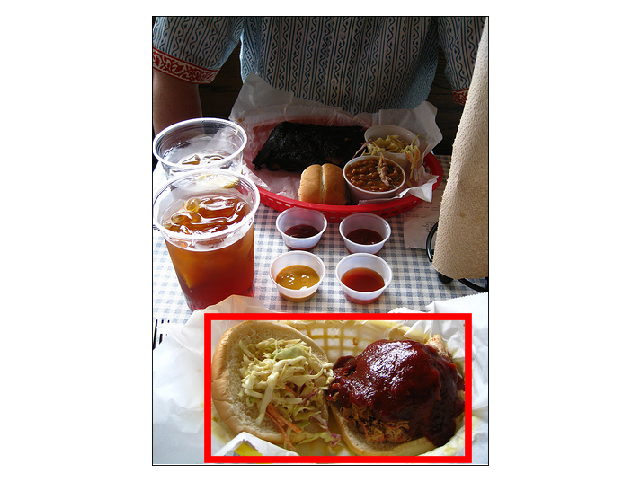
\includegraphics[width=0.9\linewidth]{figures/2379889_1353176_supercat_unique.png}}  sandwich (15), basket (6), food (5), burger (2), hamburger (2), meal (2) &
\raisebox{-\totalheight}{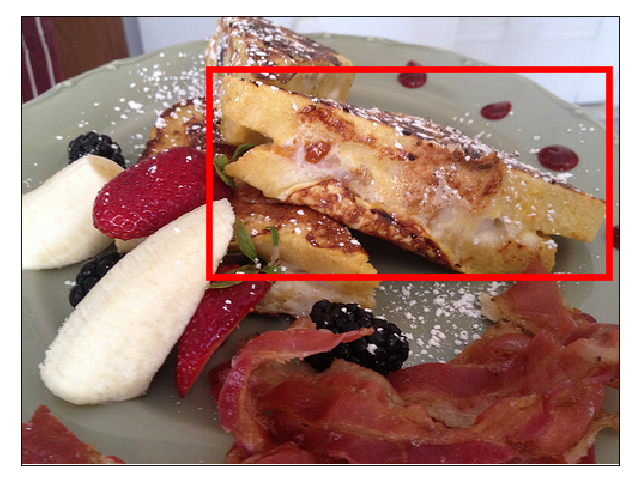
\includegraphics[width=0.9\linewidth]{figures/2394266_465678_singleton_obj.png}} food (10), sandwich (8), toast (5), french toast (4), dessert (2), breakfast (2) &
\raisebox{-\totalheight}{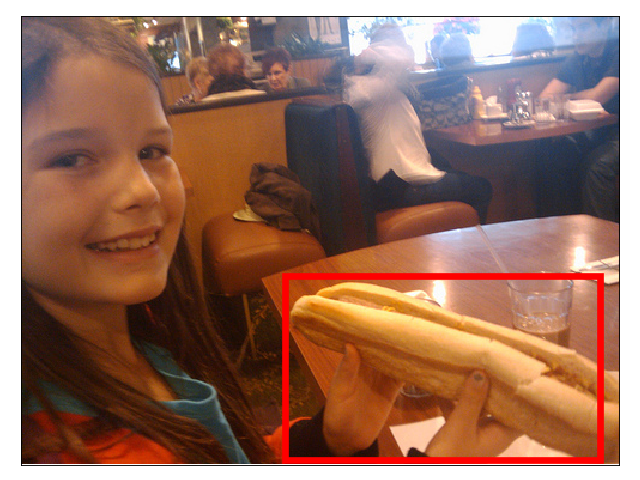
\includegraphics[width=0.9\linewidth]{figures/2386509_681763_supercat_unique.png}} hotdog (14), food (7), bun (4), sandwich (3), bread (2)\\ 
\multicolumn{4}{c}{\textbf{VG: bridge} }\\ 
\raisebox{-\totalheight}{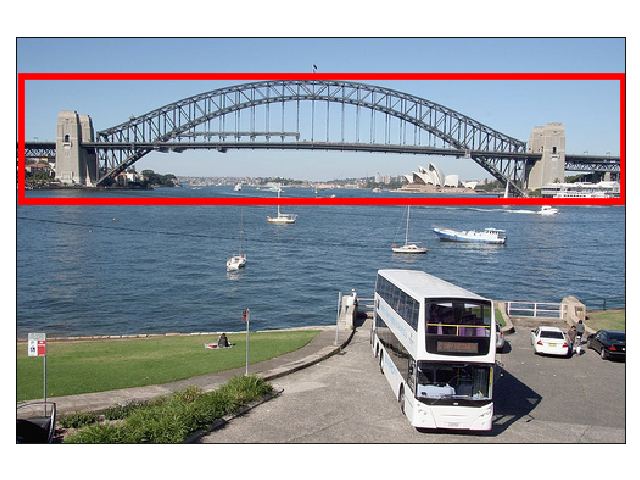
\includegraphics[width=0.9\linewidth]{figures/2341667_2006329_singleton_obj.png}} bridge (35)  &
\raisebox{-\totalheight}{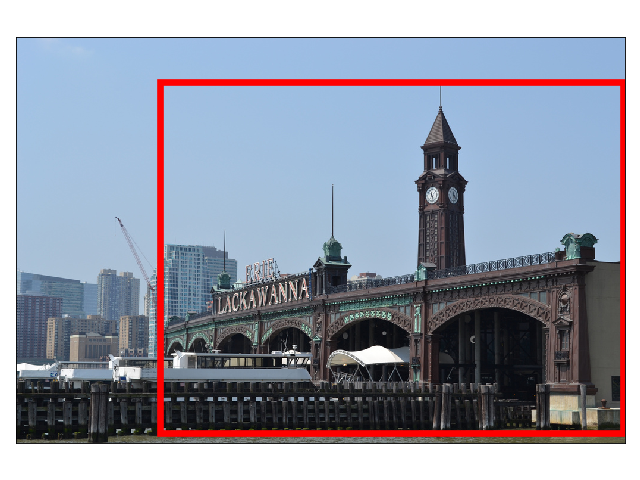
\includegraphics[width=0.9\linewidth]{figures/1592509_1610006_singleton_obj.png}} bridge (20), building (11)  &
\raisebox{-\totalheight}{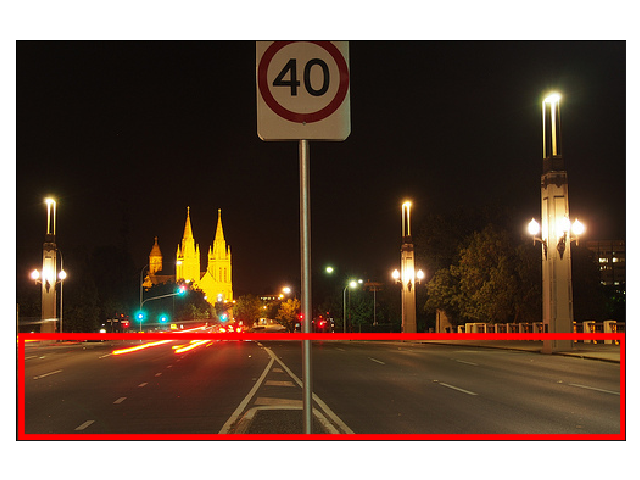
\includegraphics[width=0.9\linewidth]{figures/2384683_1306430_singleton_obj.png}} street (16), road (15), bridge (3) &
\raisebox{-\totalheight}{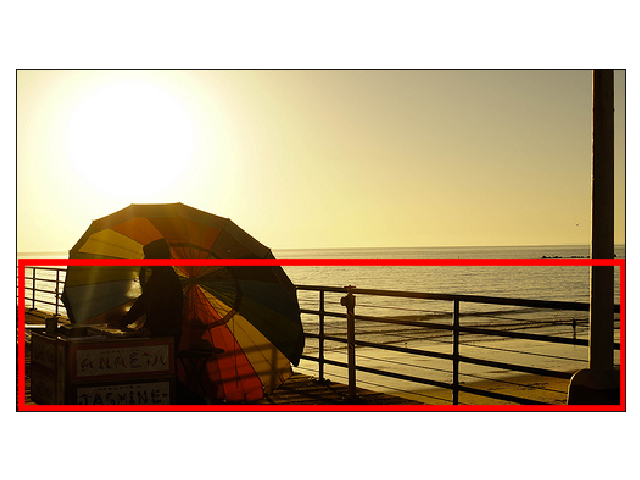
\includegraphics[width=0.9\linewidth]{figures/2412972_3494120_singleton_obj.png}} pier (6), railing (5), dock (5), bridge (5), fence (4), rail (3), boardwalk (3)\\ 
\multicolumn{4}{c}{\textbf{VG: bed}}\\ 
\raisebox{-\totalheight}{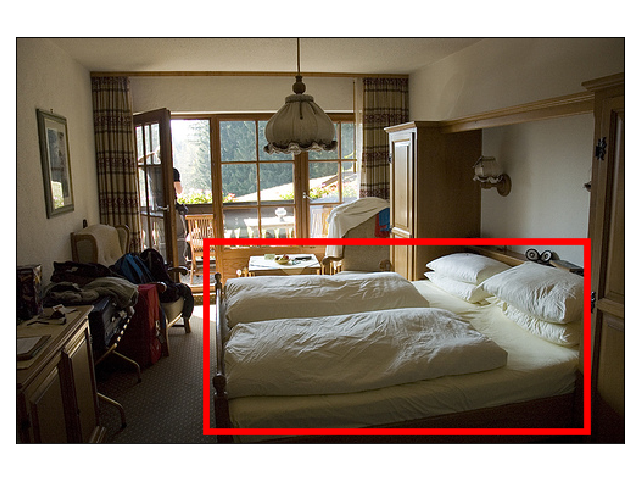
\includegraphics[width=0.9\linewidth]{figures/2321254_3438076_singleton_obj.png}} bed (36)  &
\raisebox{-\totalheight}{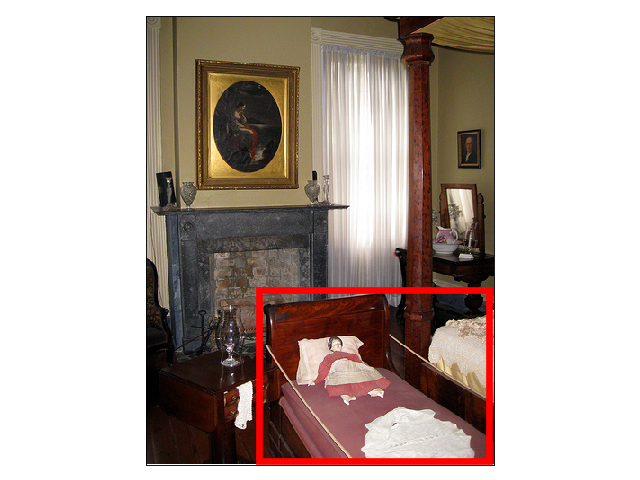
\includegraphics[width=0.9\linewidth]{figures/2324306_3412337_singleton_obj.png}}  bed (16), bench (6), crib (5) &
\raisebox{-\totalheight}{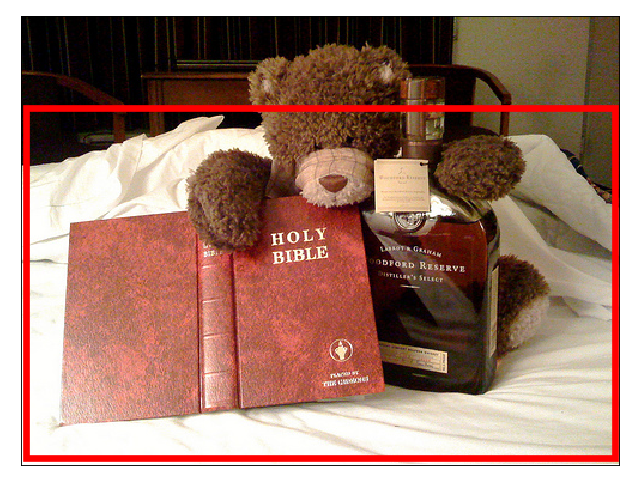
\includegraphics[width=0.9\linewidth]{figures/2342811_3485104_singleton_obj.png}}  bed (17), book (6), table (4), toy (3), bible (2), doll (2) & 
\raisebox{-\totalheight}{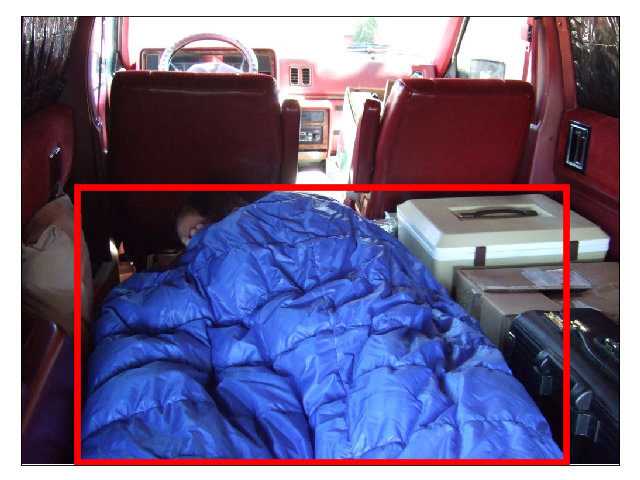
\includegraphics[width=0.9\linewidth]{figures/498222_3135415_singleton_obj.png}} bed (12), sleeping bag (9), blanket (7), bed sheet (5)\\ 
\multicolumn{4}{c}{\textbf{VG: batter}}\\
\raisebox{-\totalheight}{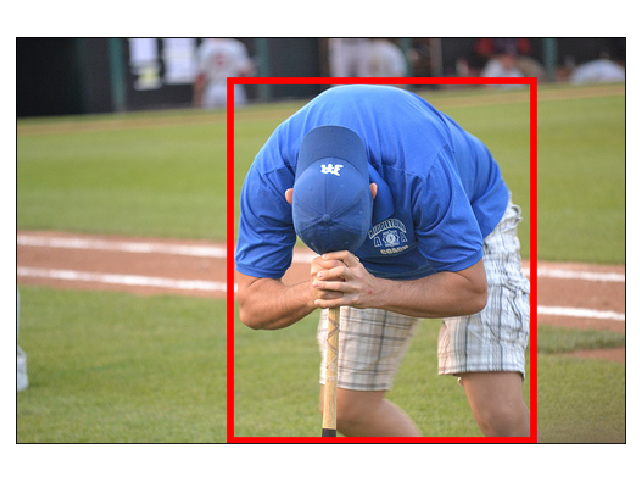
\includegraphics[width=0.9\linewidth]{figures/2372219_2683892_supercat_unique.png}} man (24), cap (5), person (3), baseball player (2) &
  \raisebox{-\totalheight}{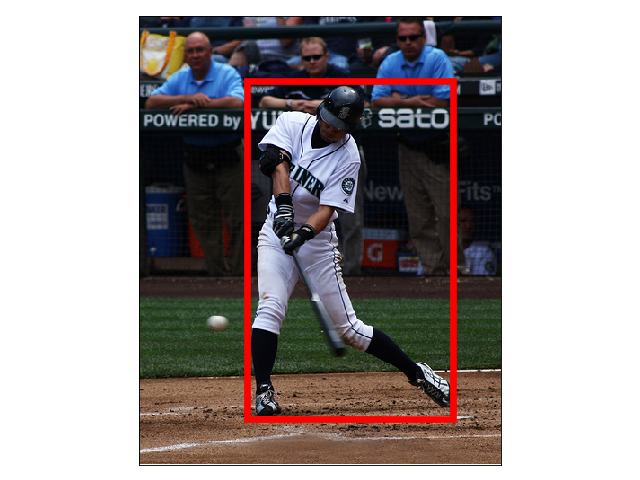
\includegraphics[width=0.9\linewidth]{figures/2394377_464684_singleton_obj.png}} man (13), baseball player (7), batter (5), player (3), helmet (2) &
\raisebox{-\totalheight}{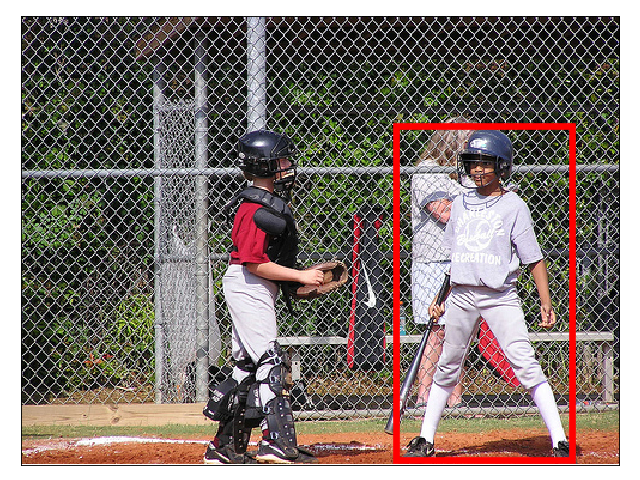
\includegraphics[width=0.9\linewidth]{figures/2398907_2901496_singleton_obj.png}}  boy (7), helmet (5), baseball player (4), player (4), man (3), child (3), batter (3), dress (2), kid (2)&
\raisebox{-\totalheight}{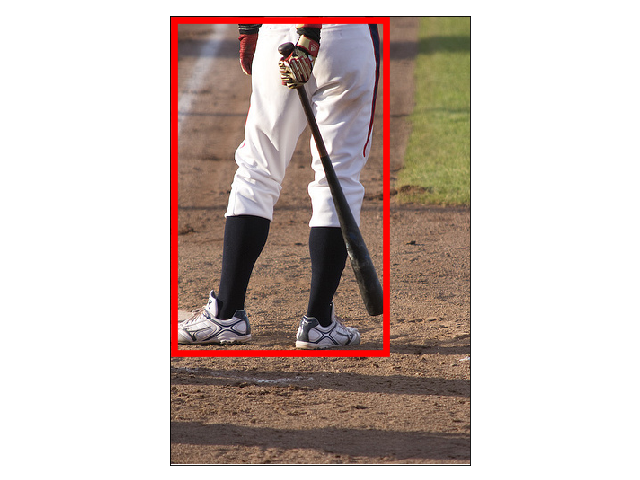
\includegraphics[width=0.9\linewidth]{figures/2337552_957263_singleton_obj.png}} pants (6), player (5), shoe (4), bat (4), person (4), legs (4), baseball player (3), hitter (2)\\ 
\multicolumn{4}{c}{\textbf{VG: robe}}\\
\raisebox{-\totalheight}{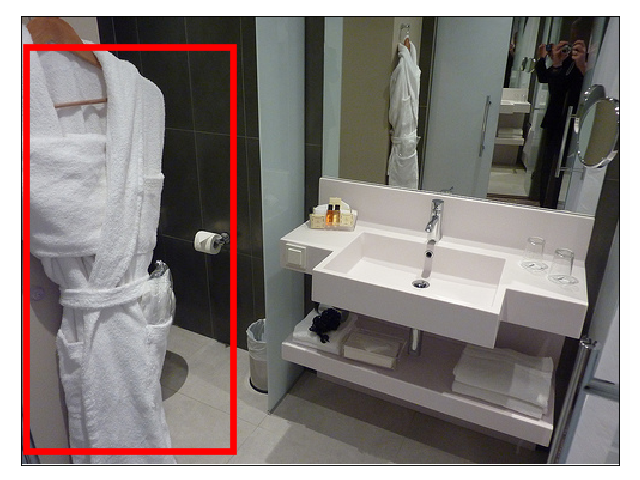
\includegraphics[width=0.9\linewidth]{figures/2373180_2333161_singleton_obj.png}} robe (27), bathrobe (5) &
  \raisebox{-\totalheight}{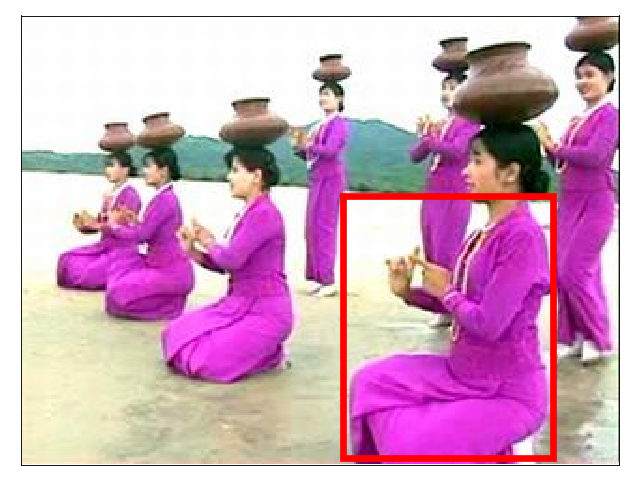
\includegraphics[width=0.9\linewidth]{figures/160_1058761_supercat_unique.png}} dress (30), uniform (2) &
\raisebox{-\totalheight}{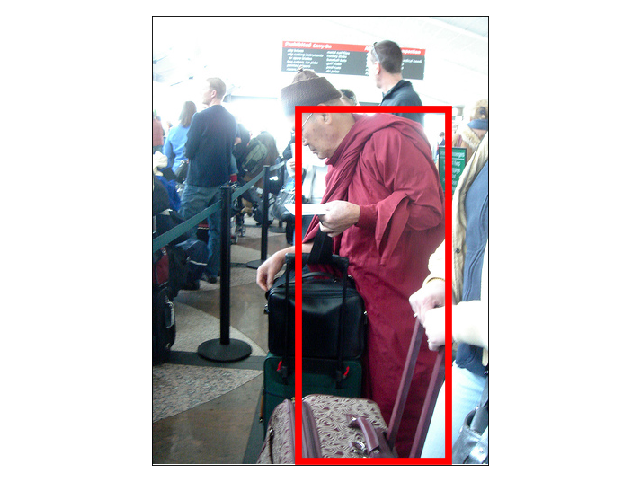
\includegraphics[width=0.9\linewidth]{figures/2334612_2838713_supercat_unique.png}}  robe (11), jacket (7), clothes (6), bag (3), dress (2), man (2) &
\raisebox{-\totalheight}{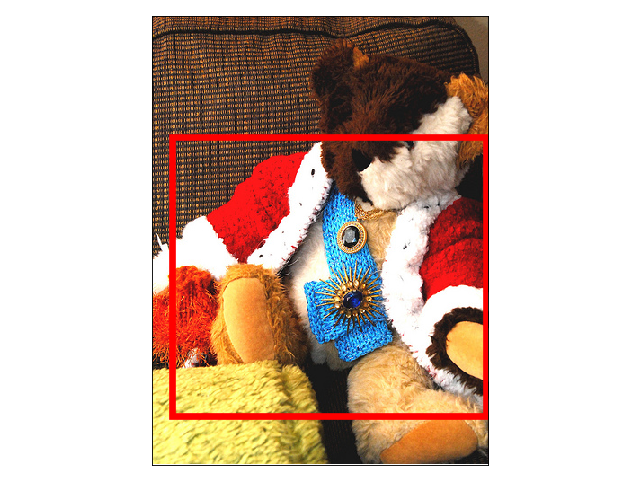
\includegraphics[width=0.9\linewidth]{figures/2340041_2137546_supercat_ambiguous.png}} jacket (10), sweater (9), coat (3), doll (3), toy (3), shirt (2), bear (2), robe (2)\\ 


\end{tabular}

}
\end{minipage}

 \caption{\label{fig:ex}Examples for different instances of VG synsets with low and high agreement in MN data set}
\end{figure*}



%\gbt{The non-canon. VG names suggest that people prefer more general names (``car $>$ sedan'', ``horse $>$ pony'', ``tie $>$ necktie''). Could be due to lexical availability (more general \ra more frequent \ra more available). This could be verified (using frequency). Hypothesis: In cases where top name != VG, the VG name is less general. Could be also a more general hypothesis: see if people prefer more frequent names in general.}
%\cs{@Table~\ref{tab:qual} (just wrt presentation) The most interesting blocks are 2 and 3 (canonical VG with min agr.; non-canonical with max agr.)}


\subsection{Discussion (for now)}
What does this discrepancy between the instance-level and category-level agreement in VisualGenome and ManyNames naming choices mean? 
First of all, it suggests that the same original VisualGenome name can trigger very different variants depending on the visual instance, leading to a drastic increase of variants elicited for categories as compared to instances.
Second, this clearly shows that annotators in VG do not generally annotate the most canonical name \cs{but they don't annotate the name, but the description} and that many names annotated for objects in VG do not correspond to the overall most preferred variant. \sz{think more ...}
\gbt{I don't think we can conclude this second part -- we do have the 70\% top=VG figure that says that VG annotators annotate the most canonical name. What this suggests to me is that instance-level properties are more important than category-level properties, somehow.
  That is, there are systematic properties of instances that make them have a single most salient name.
  However, I expect that this result will be very influenced by referential uncertainty (in single images, it will mostly be clear that it's a man, but in some it may be unclear \ra high instance agreement, low category agrement.}
\cs{I don't think that 70\% is high. E.g., the ResNet has a top-1 error rate of 25\% on ILSVRC 2015.}

\cs{(?!?) With respect to implications for L+V  models on language *interpretation*: much lower agreement on object class-level than on instance-level speaks for using very fine-grained object annotations (as done in ILSVRC). 
	However, that naming variants are often not explained/recoverable by hierarchical relations questions in how far models can understand/interpret reference to objects using more general classes (i.e., names), despite being able to recognise an object's very specific class (e.g., ILSVRC synset). (Relevant?!?)}

\begin{table*}
\footnotesize
%\begin{tabular}{p{1.3cm}cccccc|cccccc}
%\toprule
% & \multicolumn{6}{c|}{Instance-level agreement} & \multicolumn{6}{c}{Class-level agreement}\\ 
%           domain & \% top &    $H$ &    N & N$_{>1}$ & top=VG &  \% VG & \% top &    $H$ &     N & N$_{>1}$ & top=VG &  \% VG \\
%\midrule
%            all &  69.7 (22.2) &  1.3 &  5.7 &   2.9 &  72.8  &  58.7  &   52.6 (21.1) &  2.4 &   62.2 &  29.7 &  32.7 (46.9) &  23.5 (27.0)  \\
% \midrule
%         people &  51.9 (18.1) &  2.1 &  8.6 &   4.3 &         49.8 &         32.3 &     43.1 (14.9) &  2.9 &  104.4 &  53.4 &         24.4 &         13.2  \\
% animals\_plants &  91.3 (12.9) &  0.4 &  2.7 &   1.5 &         93.8 &         88.0 &     67.9 (23.5) &  1.5 &   26.7 &  12.4 &         29.5 &         26.2  \\
%       clothing &  63.9 (17.9) &  1.6 &  6.4 &   3.2 &         70.2 &         52.6 &     49.3 (16.6) &  2.6 &   71.7 &  34.1 &         40.5 &         26.1  \\
%       vehicles &  72.0 (19.5) &  1.1 &  4.7 &   2.4 &         71.1 &         60.2 &    54.4 (17.4) &  2.1 &   70.4 &  33.2 &         21.4 &         21.3  \\
%      buildings &  66.9 (20.5) &  1.5 &  6.9 &   3.0 &         72.6 &         55.5 &      46.7 (18.2) &  3.0 &   68.5 &  31.3 &         32.3 &         22.3  \\
%           home &  66.4 (20.5) &  1.5 &  6.3 &   3.1 &         78.5 &         58.8 &     49.6 (18.7) &  2.8 &  103.2 &  48.8 &         45.9 &         30.1  \\
%           food &  71.3 (21.1) &  1.3 &  5.5 &   2.9 &         62.9 &         52.1 &     47.3 (19.5) &  2.5 &   32.1 &  15.2 &         31.1 &         20.8  \\
%\bottomrule
%\end{tabular}

\begin{tabular}{lccccc|ccccc}
\toprule
 & \multicolumn{5}{c|}{Instance-level agreement} & \multicolumn{5}{c}{Class-level agreement}\\ 
          domain &    N &         \%top (std) &          H (std) & top=VG &   \%VG &     N &         \%top (std) &          H (std) & top=VG &   \%VG \\
\midrule
            all &  2.9 &  75.2 (21.9) &  0.9 (0.7) &   72.8 &  62.8 &  29.7 &  56.4 (21.5) &  2.0 (1.0) &   32.7 &  23.4 \\
       vehicles &  2.4 &  76.6 (19.8) &  0.8 (0.6) &   71.1 &  63.9 &  33.2 &  57.4 (17.3) &  1.8 (0.6) &   21.4 &  21.2 \\
      buildings &  3.0 &  74.7 (20.7) &  1.0 (0.7) &   72.6 &  61.6 &  31.3 &  51.0 (18.8) &  2.4 (0.9) &   32.3 &  22.2 \\
       clothing &  3.2 &  70.1 (18.5) &  1.1 (0.6) &   70.2 &  57.4 &  34.1 &  53.4 (16.6) &  2.1 (0.8) &   40.5 &  26.1 \\
           home &  3.1 &  72.6 (20.7) &  1.0 (0.7) &   78.5 &  64.1 &  48.8 &  54.0 (19.4) &  2.3 (1.0) &   45.9 &  29.9 \\
         people &  4.3 &  59.0 (20.4) &  1.5 (0.7) &   49.8 &  36.3 &  53.4 &  47.5 (17.2) &  2.5 (0.9) &   24.4 &  13.0 \\
           food &  2.9 &  76.4 (20.7) &  0.9 (0.7) &   62.9 &  55.2 &  15.2 &  50.8 (20.3) &  2.0 (0.8) &   31.1 &  20.8 \\
 animals\_plants &  1.5 &  94.5 (12.1) &  0.2 (0.4) &   93.8 &  91.0 &  12.4 &  71.3 (23.3) &  1.2 (0.9) &   29.5 &  26.1 \\
\bottomrule
\end{tabular}

\caption{Agreement in naming measured on the level of instances and on the level of VG classes (i.e.\ after grouping objects by their VG synset), for filtered response sets (frequency threshold of 2)}
\label{tab:agree}
\end{table*}


%Why is naming more flexible in certain domains than in others? \gbt{Hypothesis: expectation: little variation - hypernymy at most, more variation <-> more affordances <-> more varied relationships.}



\cs{@Table~\ref{tab:agree} I still think that we could also have \%\ top with $N>1$ to give an idea as to how useful the data is for the people interested in using it for, e.g., model evaluation. For that, it is clear that crowdsourcing is noisy and before using it some outlier removal needs to be made.}

% \subsection{Entry-level names and preference orders....}

% \sz{an interesting example:} In our data set, there are 24 images where \textit{penguin} has been used, so we know that the object is a \textit{penguin}. For 50\% of these images, annotators still prefer \textit{bird} as the most common name. According to the theory of entry-level categories, this should not happen. People should always prefer \textit{penguin} over \textit{bird}. 

% \sz{how can we analyze this quantitatively?}

% \begin{itemize}
% \item lettuce -- salad
% \item fruit -- food
% \item man -- catcher
% \item bowl --chili
% \item bowl -- diner \gbt{spelling mistake? should be dinner?} 
% \item burger -- meat
% \item statue -- animal (image shows statue of an animal)
% \item bottle -- alcohol
% \item donut --desert \gbt{spelling mistake? should be dessert?} 
% \item zebra -- stripes
% \item oven -- grill
% \end{itemize}


%%% Local Variables:
%%% mode: latex
%%% TeX-master: "main"
%%% End:


Probably largely same content; make sure that the analysis bears on the question, ``to what extent do current L\&V models account for human naming behavior?''. And that it is cohesive.

\bibliographystyle{acl_natbib}
\bibliography{naming}
\end{document}

%%% Local Variables:
%%% mode: latex
%%% TeX-master: "acl2020_main"
%%% End:
